\documentclass[
	11pt,
	toc=bibliography
	]{article}
\usepackage{array} % for defining a new column type
\usepackage{varwidth} %for the varwidth minipage environment
\usepackage{caption}
\usepackage{adjustbox}
\usepackage{longtable}
\usepackage{graphicx}
\usepackage{tabulary}
\usepackage[a4paper, total={6in, 8in}]{geometry}
\usepackage[table,dvipsnames]{xcolor}
\usepackage[
	hidelinks,
	colorlinks,
	allcolors=black,
	bookmarks=true	
	]{hyperref}
\usepackage[
	numbered,
	open,
	openlevel=1
	]{bookmark}
%\usepackage[pages=all]{background}
\usepackage[firstpage=true]{background}
\backgroundsetup{
scale=1,
color=black,
opacity=0.4,
angle=0,
contents={%
  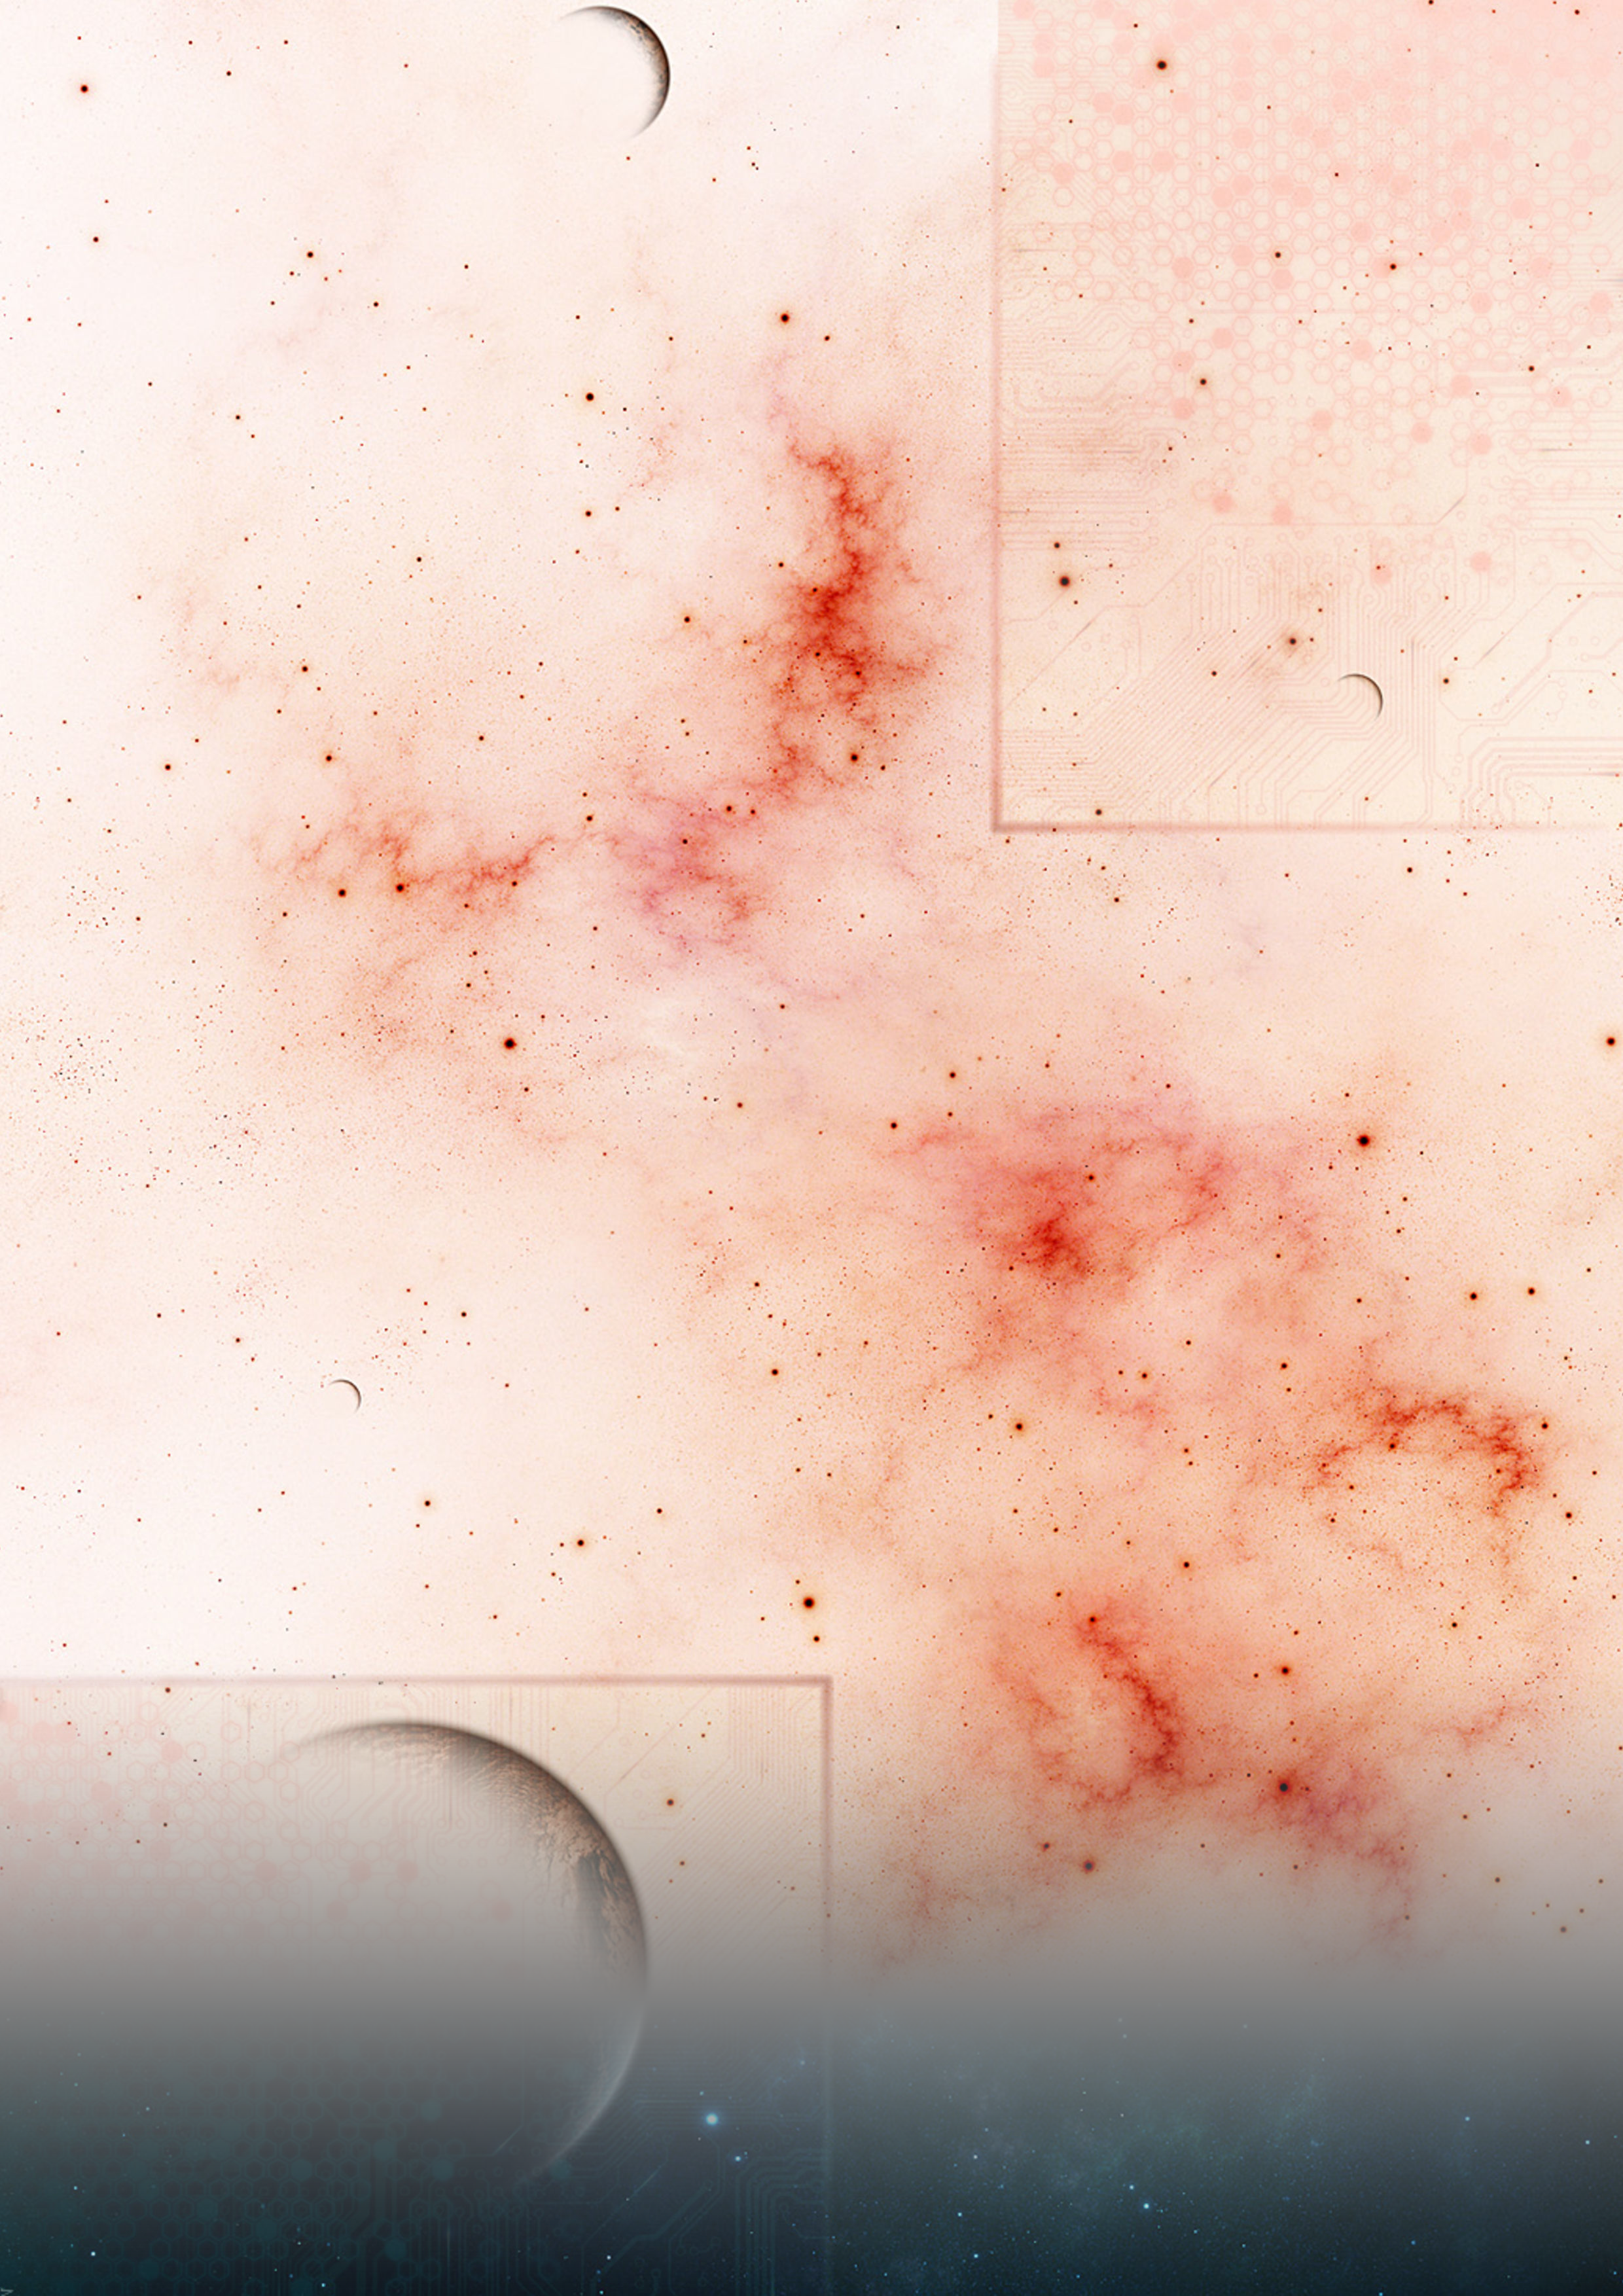
\includegraphics[width=\paperwidth,height=\paperheight]{Background2}
  }%
}

%   Pakete dazuladen
\usepackage{titlesec} % defining font styles for sections etc

\titleformat{\section}
{\normalfont\scshape}{\thesection}{1em}{}[\vspace{2ex}\titlerule]

\titlespacing{\section}{-45pt}{10ex plus 1ex minus .2ex}{4.3ex plus .2ex}

\newcommand{\sectionbreak}{\clearpage}

\titleformat{\subsection}
{\huge\bfseries}{\small\thesubsection}{.8em}{}

\titlespacing{\subsection}{0pt}{8ex plus 1ex minus .2ex}{1ex plus .2ex}


\usepackage{array} % for defining a new column type
\usepackage{varwidth} %for the varwidth minipage environment
\usepackage{caption}
\usepackage{adjustbox}
\usepackage{longtable}
\usepackage{graphicx}
\usepackage{tabulary}
\usepackage[a4paper, total={6in, 8in}]{geometry}
\usepackage[table,dvipsnames]{xcolor}
\usepackage[
hidelinks,
colorlinks,
allcolors=black,
bookmarks=true	
]{hyperref}
\usepackage[
numbered,
open,
openlevel=1
]{bookmark}
%\usepackage[pages=all]{background}
\usepackage[firstpage=true]{background}
\backgroundsetup{
	scale=1,
	color=black,
	opacity=0.4,
	angle=0,
	contents={%
		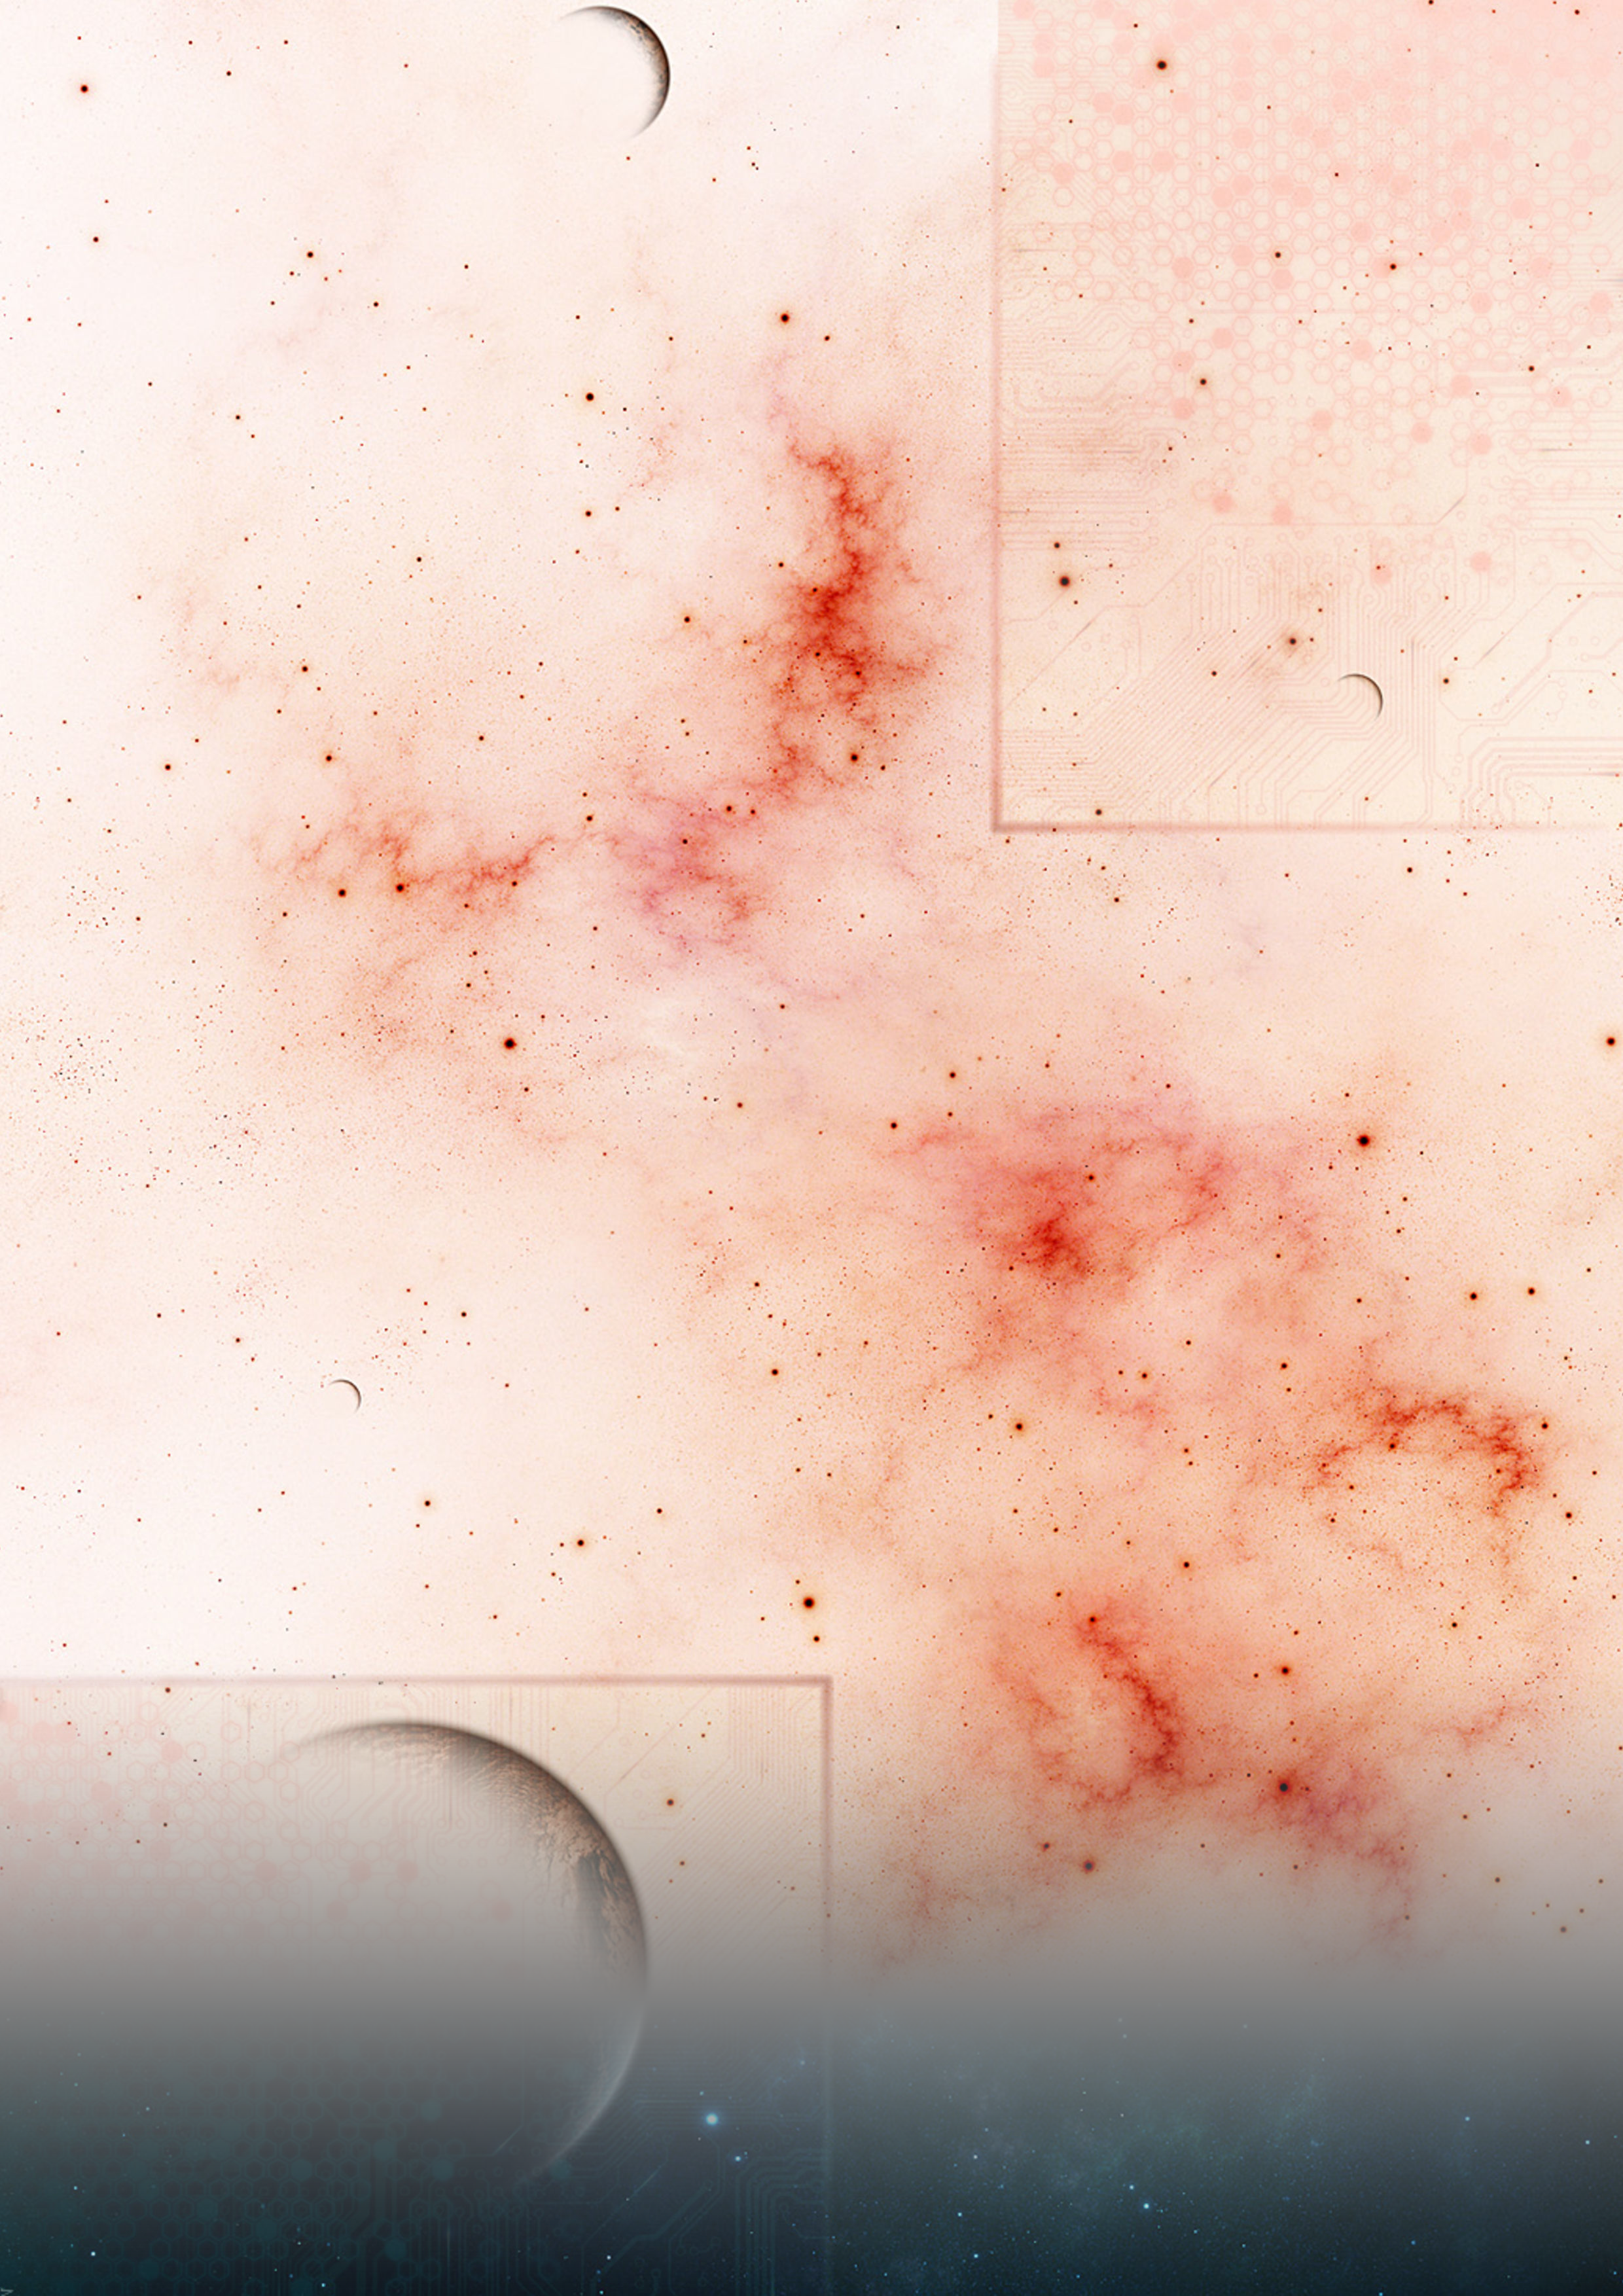
\includegraphics[width=\paperwidth,height=\paperheight]{Background2}
	}%
}

%   Schriftart der auf den Karten eingesetzten Texte
\usepackage{anttor}

%   UTF-8 Encoding der TeX-Dateien
\usepackage[utf8]{inputenc}

%   englisches Sprachpaket
\usepackage[english]{babel}

%   optischer Randausgleich
\usepackage{microtype}

\usepackage{color}

%   TikZ zum "Malen" von Grafiken, in diesem Falle für die Karten
\usepackage{tikz}
\usetikzlibrary{patterns}
\usetikzlibrary{shadows}

%   Symbole dazuladen; Verwendung \ding{<nummer>}
\usepackage{pifont}
%   weitere Symbole
\usepackage{fourier-orns}
%   Farbdefinitionen laden
%   FARBEN DER ELEMENTE/BESTANDTEILE DER KARTEN
%   -----------------------------------------

%   Hintergrundfarbe für den Titel-Kasten
    \definecolor{titlebg}{RGB}{30,30,30}

%   Farben der "Fähnchen" zur Kennzeichnung der unterschiedlichen Kartentypen
    \definecolor{damagebg}{RGB}{100,150,150}
    \definecolor{criticaldamagebg}{RGB}{200,50,50}
    \definecolor{missionbg}{RGB}{80,100,50}
    \definecolor{testbg}{RGB}{150,150,150}
    
    \definecolor{black}{RGB}{0,0,0}

%   Farbe des "Fähnchens" zur Angabe des Preises der Karten
    \definecolor{pricebg}{RGB}{230,180,0}

%   Hintergrundfarbe für den Textbereich
    %\definecolor{content}{RGB}{250,250,245}
    \definecolor{contentbg}{RGB}{255,255,255}
%   \card-Commands laden
\input{tikzcards.tex}



\newcommand{\myparagraph}[1]{\paragraph{#1}\mbox{}\\}

\begin{document}
%\BgThispage
\newcolumntype{M}{>{\begin{varwidth}{4cm}}l<{\end{varwidth}}}

\phantomsection \pdfbookmark{First Page}{first page}
\title{Between two Suns}
\maketitle

\cleardoublepage\phantomsection\pdfbookmark{Contents}{contents}
\tableofcontents
\newpage
\section{Abbreviations}\label{abbreviations}
Here you will find a couple of abbreviations that you might encounter while reading this ruleset.
\captionof{table}{Abbreviations}
\begin{tabular}[t]{lll}
&&\cr\\
Mov & = & Movement \cr\\
Mel.S & = & Melee Skill \cr\\
Aim & = & Aim Skill\cr\\
S & = & Strength \cr\\
T & = & Toughness \cr\\
AP & = & Action Points \cr\\
ATK & = & Number of Attacks \cr\\
WP & = & Willpower \cr\\
LD & = & Leadership / Morale \cr\\
HP & = & Health Points / Hull Points \cr\\
DP & = & Defense Penetration \cr\\
SN & = & Shield Negation \cr\\
" & = & Inch / Inches\cr\\
D6 & = & a 6-sided dice\cr\\
AoE & = & Area of Effect\cr\\
CC & = & Close Combat\cr\\
FP & = & Front Armor Plating\cr\\
SP & = & Side Armor Plating\cr\\
BP & = & Back Armor Plating\cr\\
\end{tabular}

\newpage
\section{What you need}\label{whatYouNeed}
\begin{itemize}
\item a measuring device for inches
\item several 6-sided dice (the more, the better)
\item some artillery and deviation dice (look those up, they're easy to get. If you still don't have any, they're 6-sided also, so just use regular dice and agree on which result triggers what)
\item some 3'', 5'' circle templates and a flame template
\item 1 damage deck per player(36 cards), 2 for anyone with more than 6 vehicles
\item tactical objectives deck (36 cards)
\item Action Markers (Move, Special, Shoot, Charge)
\item State Markers (Reload, Preparation, Suppressed, Suppressing, Targeted)
\end{itemize}

\section{Structure of Play}\label{structureOfPlay}
One \textit{Round} of play consists of 2 \textit{Phases}.\\
At the beginning of the game determine which player has the initiative by rolling the dice (+1 if you fielded less points than your opponent).\\
At the start of each \textit{Phase} each player chooses an Action Marker for each of his units and places it face down next to the unit. Starting with the player having the initiative, the players each reveal one unit's Action Marker and perform the chosen action. They continue in this manner until all units have performed their action. Then the next \textit{Phase} starts and the other player gets the initiative and so on.
A game last for a maximum of 6 rounds.

\subsection{The Bonus Action}\label{theBonusAction}
\textbf{Once per Round} - as long as your general is alive - you may let a unit perform an additional action. This may be done before or after you reveal and perform the unit's regular action.

\subsection{Placement of terrain and units}\label{placementTerrainUnits}
We suggest playing with at least 12 urban terrain pieces. At least 4 of them should be bigger ones like buildings and such. Place them as you wish or randomly but especially the unit placement zones of each player should be free of any buildings but still provide a roughly equal amount of cover.\\\\
The unit placement zones should have a distance of 30'' to each other. Players take turns placing their units. After placement is completed roll a dice, the player with the highest result gets the first turn.

\subsection{Possible Actions}\label{possibleActions}
Each type of action may be performed only \textbf{once per round} by each unit. This remains true even for \textit{The Bonus Action} (chapter \ref{theBonusAction}).
\rowcolors{2}{gray!25}{white}
\captionof{table}{Possible Actions}
{\renewcommand{\arraystretch}{2}
\begin{longtable}{V{.32\textwidth} V{.62\textwidth}}
\rowcolor{gray!50}
\bf Action Type & \bf Description \\ 
\hline 
Movement & Move the unit in any way and direction according to your movement value (Mov). May not be used to initiate CC.\\ 
Special & Use Abilities and Items with the \textit{Special} Rule (Biotic, Grenades, Overwatch, Reload, etc.).\\ 
Charge & Move the unit in any way and direction for half of its Mov (rounded up) + D6. May initiate \textit{CC}.\\ 
Shoot & Shoot with one equipped weapon of your choice (Or shoot with one Weapon Pair/synchronized Weapon System)\\ 
Prepare & The unit gains one Preparation Token (Is lost again if the unit does any action that does not cost a Preparation Token)\\
\end{longtable}}

\subsection{Moving a Squad}\label{movingASquad}
Individual squadmembers must always have another squadmember inside the range of 1,5'' again after moving.

\subsection{Initiating Close Combat}\label{initiatingCloseCombat}
Charging into base contact with an enemy unit \textit{initiates Close Combat}. This is only possible if the enemy unit has already been seen at the start of the Charge, otherwise the movement may not take you closer than 2'' to an enemy unit. \\
A successful CC initiation will trigger one round of CC and render all participating units unusable for the rest of the Phase.\\\\
If one model is in CC with another unit, all the other models of this unit will automatically use their Mov in their next Phase to join the fray. This doesn't apply if they're already bound by another CC.\\

\subsection{Being bound by Close Combat}\label{beingBoundByCloseCombat}
Units \textit{bound by Close Combat} may only choose to continue their CC and therefore don't get any Action Markers at the start of each Phase. Any of the players may choose his/her unit \textit{bound by Close Combat} like he/she would to reveal their Action. This will trigger one round of CC and render all participating units unusable for the rest of the Phase.\\\\
A unit stays \textit{bound by Close Combat} until one side is either wiped out, has fled or removes itself/is removed from the CC otherwise.\\\\
Vehicle models that are engaged in CC cannot be bound by it and may perform Actions as they normally would. If they choose to fire their light weaponry however, they may only target the unit they are currently engaged with in CC. Heavy Weaponry may still target everything according to its regular rules (see Chapter \ref{weaponry}, Heavy Weaponry). If they decide to drive out of the Close Combat and end it this way, they will receive one automatic hit from every model in base contact. For further Information on vehicles consult the vehicle chapter \ref{vehicles}. 

\subsection{Rules of Sight}\label{rulesOfSight}
We're using a ''real line of sight'' starting on the height of the eyes of the model.\\
Every model has a 180 degree field of view.\\
In a 5'' circle around the model it even has a 360 degree field of view.\\
What is seen and what is not seen is determined once right before every action the unit takes.

\subsection{Sizes}\label{sizes}
Models can have one of four distinct sizes.
\rowcolors{2}{gray!25}{white}
\captionof{table}{Possible Actions}
{\renewcommand{\arraystretch}{2}
\begin{longtable}{V{.1\textwidth} V{.25\textwidth} V{.2\textwidth} V{.25\textwidth}}
\rowcolor{gray!50}
\bf Size & \bf Affected Units  & \bf Base Size & \bf Cover granted from\\ 
\hline 
Size 0 & Everything that's about half-a-human big & 25mm round& All sizes. Additionally treats any kind of cover as heavy cover when getting shot at\\ 
Size 1 & Roughly human-sized & 25mm round & All sizes\\ 
Size 2 & Considerably bigger than a human (Cyborg, Werewolf, etc.) & 40mm round & Objects or units size 1 or bigger\\
Size 3 & Even bigger than that (Cybots, Mechs, etc.) & 60mm round & Objects or units size 2 or bigger\\ 
Size 4 & Really big (Tank, Brain Bug, Elephant, you name it) & 105mm*70mm oval (or bigger if the model is bigger) & Objects or units size 3 or bigger\\ 
\end{longtable}}

\section{Shooting, Hitting, Wounding, Saving, Killing and other related fun}\label{combatSystem}
In this section you're going to learn about the combat system in Between two Suns. We went for a relatively sophisticated approach that allows both players to influence it at many stages and furthers the fun of butting your heads against each other. Without further ado, let's get started.

\subsection{Shooting and Hitting in Ranged Combat}\label{theShootyPart}
\subsubsection{Whom to Shoot at}\label{whomToShoot}
You may only shoot at \textbf{entire units} (Squad, Hero, Commander, Vehicle, etc.) if not noted otherwise.\\\\ 
Your shooting model must be able to see the unit it wants to shoot at at least partly when beginning to shoot \textit{(only seeing a finger/part of a knee/a little bit of the 10 foot standard they're carrying around doesn't count you nitpickers!)}. \\
Even if you have seen only one model out of a whole unit, you may still decide to shoot at the whole unit, but the cover rating of the majority of the squad always applies. \\
When you are actually shooting at a singular model, only its own cover rating applies.

\subsubsection{Shooting Area of Effect Weapons}\label{shootingAoEWeapons}
If firing an Area of Effect Weapon you throw the artillery and the deviation dice and substract the shooters aim from the result to correct the shot (If not specified otherwise in the rules of the weapon). Then deviate the shot according to the result.\\
''Hit'' Symbols on the dice have no effect. \\
If you roll a ''Misfire'' Symbol, then you have to reroll the deviation distance and this time you aren't allowed to correct it with your aim. If you happen to roll a second Misfire on this try, this shot and all remaining shots from this weapon are lost for this turn. 

\subsubsection{Indirect Fire}\label{indirectFire}
Area-of-Effect Weapons that fire using the above method (no shotguns, flamethrowers etc.) are able to fire indirectly if they would have the possibility to fire at their target but cannot see it (because it’s behind a building for example) \textbf{and} another friendly unit has line of sight on their target. If firing indirectly every shot is handled as if a misfire symbol had been rolled previously (no aim correction and a misfire symbol means no shot).

\subsubsection{Hitting those Shots from afar}\label{hittingRanged}
For every shot you take throw a D6. If the result is the same or higher than 7-Aim (use the Aim of the shooter) then the shot is a hit. A rolled 1 is always a miss.\\
Your Aim will be modified by the difficulty of the shot and can even become negative!\\
If you'd have to roll a 7,8 or 9 to hit you may do this by rolling a 6 first and then a 4,5 or 6 after.\\
If you'd have to roll higher than a 9 to hit, the shot is impossible and cannot be taken.\\
Here are the Aim modifcations your shooter may experience:
\rowcolors{2}{gray!25}{white}
\captionof{table}{Possible Aim Modifications}
{\renewcommand{\arraystretch}{2}
\begin{longtable}{V{.3\textwidth} V{.14\textwidth} V{.5\textwidth}}
\rowcolor{gray!50}
\bf Name & \bf Effects AoE Weaponry & \bf Modifications \\ 
\hline 
Light Cover & No & -1 Aim for the shooter and +1 T for the target (fences, bushes,etc.), see chapter \ref{terrainCharacteristics} for information about cover and AoE weaponry \\ 
Heavy Cover & No & -2 Aim for the shooter and +2 T for the target (walls out of stone, metal, etc.), see chapter \ref{terrainCharacteristics} for information about cover and AoE weaponry\\ 
Multiple Cover Objects & No & Multiple cover objects in the line of the shot will always add up to the effects of Heavy Cover, no matter their own cover rating \\ 
Last quarter of the weapon range (rounded up) & Yes & -1 Aim for the shooter\\
Shooting while being suppressed & Yes & -2 Aim for the shooter\\
Shooting on infantry or vehicles that have used Charge & Yes & -1 Aim for the shooter\\
Shooting at a target size 3 or bigger & Yes & +1 Aim for the shooter\\ 
Shooting at a singular infantry model & No & -1 Aim for the shooter (-2 if the target belongs to a squad)\\
\end{longtable}}

\subsubsection{Shooting at Squads}
If you shoot at a squad you throw a D6 for every hit you've caused to determine randomly which part of the squad got hit. Keep in mind the unit's constellation though. The damage against the regular soldiers gets determined first, since the Squadleader and Specialist might lose their Careful! Save (see chapter \ref{careful!}).\\\\

\textit{Example: Pete has a GI Squad with 4 regular GIs and a Specialist as well as a Squadleader. If he gets shot at by some \textbf{crazy muthafucka} his regular soldiers would get hit on 1-4, his Specialist would get hit on a 5 and his Squadleader would get hit on a 6.}

\subsection{Hitting in Close Combat}\label{hittingMelee}
A Close Combat is split in several combat groups.\\
A combat group is a blob of models being in base contact and slashing away at each other.\\
Models that are not in direct basecontact with an enemy model do not participate in this round of combat calculations. They do however still count as being bound by Close Combat and participate in post combat calculations like for example morale tests.\\
Combat calculations are done seperately for each combat group.\\
Every model in the Close Combat gets an attack run.\\
Models that charged this turn always act first. In all other cases the initiative order gets defined by the highest Mov+Mel.S combination.\\
Models that are killed before they get to act loose out on their attack run, since they're dead.\\
Models with the same Initiative do their attack runs at the same time and may very well kill each other in the process.\\\\
\textbf{Now let's get to the actual attack}\\
The model making its attack run decides how to split up its attacks given in its ATK stat between the enemies in basecontact.\\\\
The attacking model will \textit{set the level} of each attack and defending models will have to \textit{reach that} with their parry.\\\\
The attacking model throws a D6 for every attack it makes at an enemy and adds its Mel.S to each of the dice. The results will be the level of each attack. To parry an attack, the defender has to make a parry of the same or higher level.\\
In order to try this, the defending model throws as many D6 as there are incoming attacks to parry, but it may only add its Mel.S to as many dice \textbf{per turn} as itself has ATK.\\ \textit{The ATK stat stands for the number of attacks a model can dish out per turn \textbf{and} for the number of attacks a model can properly defend against per turn. It may have to defend itself against more attacks than that, but it will have a hard time doing so.}\\\\
\textbf{Parry rolls of 1 are automatically failed parries}. This stays the same regardless of how much Mel.S you add on to this roll.\\
\textbf{Parry rolls of 6 are automatically successful parries}.This stays the same regardless of how much Mel.S you add on to this roll.\\\\
The player that has to \textit{reach that} may arrange the pairs of results to be compared to each other.\\\\
\textit{\textbf{Have an example:} \\
John attacks Pete with his 3 attacks. He rolls a 2,3 and a 6. Adding his Mel.S of 4 to that, his attack levels are 6,7 and 10.\\\\
Now Pete tries to defend and rolls a 2,4 and a 6. Since he has only ATK 2 he may only add his Mel.S of 3 to two of his rolls. He decides to add it to the 2 and 4, since the 6 is an auto-parry anyway. \\
So now his parry levels are 5,7 and auto-parry.\\\\
Now Pete arranges the pairs (since he has to \textbf{reach it}) and blocks the 10 with his auto-parry, blocks the 7 with his 7 and fails to block the 6 with his 5. So he takes one hit which will wander on and maybe become a wound later on.
}

\subsection{Saving Rolls}\label{savingRolls}
Successful hits can get negated by Saving Rolls (if your model has any).\\
There are pre-wound Saving Rolls and post-wound Saving Rolls.

\subsubsection{Pre-Wound Saves}\label{preWound}
Pre-Wound Saves can only be made after taking a hit, but before the wound roll.

\paragraph{Common Types of Pre-Wound Saves}
Here are some common types of pre-wound saves that you will encounter.

\subparagraph{Shields}\label{shields}
\textit{Condensators create an energy shield around their user to protect him/her from hits. If they take too much incoming fire, they will overload and shut down for short amounts of time. This is by far the most common method of protection, which is why you might find equipment, abilities and weaponry developed to counteract it.}\\\\
Grants a pre-wound save according to the item description but is only able to take as many hits per turn as its wearer has HP. Is the only type of save that can be lessened by SN (see chapter \ref{shieldNegation}). Is also available for vehicles, see chapter \ref{vehicles}.

\subparagraph{Barrier}\label{barrier}
\textit{Basically an iron will. An iron will complemented with hell of a lot of biotic power.\\
A Biotic can equip a barrier to protect him/her from hits, but it will get weaker with every wound the wearer suffers, since it’s hard to concentrate on your biotic abilities with a bullet hole in your chest.}\\\\
A 4+ save that gets worse by increments of one with every lost HP until a minimum of 6+ is reached. If HP are somehow regained the save gets better again until a maximum of 4+ is reached again.

\subparagraph{Hate Injector}\label{battleFrenzy}
\textit{The Fighter delves deeper into his/her frenzy with every wound he/she suffers. A wounded battle frenzied combatant gets his/her body to ignore wounds and perform tasks others would deem a miracle.}\\\\
A 6+ save that gets better by increments of one with every lost HP until a maximum of 4+ is reached. If HP are somehow regained the save gets worse again until a minimum of 6+ is reached again.

\subparagraph{Extraordinary Reflexes}
\textit{Incredibly enhanced reflexes grant the soldier the ability to deflect and evade incoming ranged fire.}\\\\
Grants the Fighter a pre-wound save against ranged non-area-of-effect hits. Caps at a 4+ maximum. Requires certain Mel.S and an energy type melee weapon.

\subsubsection{Post-Wound Saves}\label{postWound}
Post-Wound Saves can only be made after a wound was suffered. They negate the Wound instead of the hit.

\paragraph{Common Types of Post-Wound Saves}
Reachable through the special Equipment branch:
\begin{itemize}
\item Necromonger Save
\item Priest Save
\end{itemize}
Reachable through racial Traits:
\begin{itemize}
\item Increased cellular regeneration save
\end{itemize}

\subsubsection{Multiple Saves}\label{multipleSaves}
A model may only use one save pre-wound and one save post-wound, regardless of the number of saves it has available.\\ If multiple saves are available, it will automatically use only the best one.\\\\
\textit{\textbf{Have an example:}\\
A humanoid mutant (Genetically Engineered Soldier) is equipped with the shield module MK2 (4+), which protects her from hits pre-wound. She also has a her increased cellular regeneration save, which grants her a 6+ post-wound save. This combination is possible and well liked. \\\\
\textbf{Have another example:}\\
An elven-biotic is equipped with a shield module MK2 (4+ pre-wound) und has extraordinary reflexes (6+ pre-wound).  In this case he will only use his extraordinary reflexes if his shields have been previously shut down so the player should think about wether he really wants to pay for both saves or not.}


\subsubsection{Shield Negation}\label{shieldNegation}
\textit{When shields became more and more popular, people started trying to find ways around them.}\\\\
Several Weapons, Abilities and Ammunition Types have a Shield Negation value.  Hits caused by those will lessen shield pre-wound saves according to their level.\\
SN 1 = lessens shield pre-wound saves by 1\\
SN 2 = lessens shield pre-wound saves by 2\\
SN 3 = lessens shield pre-wound saves by 3\\\\
Shield saves worse than 6+ don't exist/ can't be taken.\\\\
\textit{\textbf{Have an example:}\\
A weapon hit from a weapon with SN 2 will lessen a 3+ shield save to a 5+ shield save.
}

\subsection{Converting your Hits into Wounds}\label{convertingHitsToWounds}
Non-negated hits can become wounds.\\
Wounds are not distributed evenly amongst several models, but are instead used to kill on model after the other.
Wounding in ranged an melee works the same.\\
Wounding works similar to hitting in Melee, but this time, the roles are exchanged.\\\\
The defending model will \textit{set the level} of defense its armor and toughness put up against each hit and the attacking model will have to \textit{reach that} with their attack.\\\\
The defending model throws a D6 for every non-negated hit it suffered and adds its T to each of the dice. The results will be the level of defense against each hit. To hurt the model through the defense, the attacker has to deliver an attack of equal or higher level.\\
In order to try this, the attacking model throws an equal number of D6 and adds the S and DP of its weapon the to each of the dice.\\\\
\textbf{Attack rolls of 1 are automatically failed wounds.} This stays the same regardless of how much S you add on to this roll.\\
\textbf{If you make an attack roll of 6, you may make a follow-up roll. On a 5+, the attack is an automatically successful wound.} This stays the same regardless of how much S you add on to this roll.\\\\
The player that has to \textit{reach that} may arrange the pairs of results to be compared to each other.\\\\
\textit{\textbf{Have an example:}\\
Pete has suffered 3 non-negated hits from John. He now rolls 3D6 and gets a 1,4 and a 6. Adding his magnificent T of 7 to that, his defense levels are 8,11 and 13.\\\\
Now John tries to break through this defense and rolls a 1,5 and a 6. He makes the follow up roll for the 6 and actually gets another 6 (Lucky John!), which makes this attack an auto-wound. He adds his meager S of 2 and DP of 1 and now his attack levels are auto-fail, 8 and auto-wound.\\\\
Now John arranges the pairs (since he has to \textbf{reach it}) and uses his auto-wound and auto-fail against Petes highest rolls (11 and 13), since automatic results won't be affected by the enemy dice. Also he pits his 8 against Petes 8 and deals him another wound through that. So in the end he actually dealt poor Pete 2 wounds!}

\subsection{Re-Rolls}\label{reRolls}
If a re-roll his somehow granted every dice roll may only be re-rolled once, regardless of the source of the re-roll.

\section{Morale}\label{morale}

\section{Stats, Attributes and Making Your Own Soldiers and Units}\label{statsAttributesMakingSoldiers}
%\includegraphics[width=\textwidth]{LalaDasBild}
In this section you will learn how to build your own units. We will follow along with the example of the ''Roaming Tigers'', a 4 men General Infantry Squad including a Squad Leader and a Specialist.
\subsection{Choose the Unit Type}
When building your own unit, you first have to decide which kind of unit you want to build. This will decide your Beef Budget and your equipment options and must follow the rules for army composition in chapter \ref{armyComposition}. You may choose one of the following:
\rowcolors{2}{gray!25}{white}
\captionof{table}{Possible Unit Types}
{\renewcommand{\arraystretch}{2}
\begin{longtable}{V{.3\textwidth} V{.4\textwidth} V{.2\textwidth}V{.1\textwidth} }
\rowcolor{gray!50}
\bf Name & \bf Rules & \bf Beef Budget & \bf Training \\ 
\hline 
General Infantry & Squad with 2-6 soldiers with identical gear and profile & 25 pts & 0\\ 
Commandos & Elite Squad with 2-4 soldiers with identical gear and profile & 35 pts & 1\\ 
Hero & Single Soldier, must have max HP-1 & 45 pts & 2\\ 
Commander & Single Soldier, must have max HP & 50 pts  & 3\\ 
Support - Heavy Weapon Team & Heavy Weapon platform crewed by a squad of two general infantrymen (no Squadleader/Specialist). See chapter \ref{heavyWeaponTeams} for more information & 25 pts (for the infantrymen) & 0\\ 
Support - Vehicle & Vehicle crewed by a pilot (+ gunner). See chapter \ref{vehicles} for more information & Depends on chosen crew & 0\\ 
\end{longtable}}

\textit{For the ''Roaming Tigers'' we chose General Infantry as Unit Type, which gives us a Beef Budget of 25 pts per soldier but limits us to having exactly identical soldiers in our squad (with the exception of the squadleader and the specialist, but we'll talk about those later).}

\subsection{Choose your Race}
After you chose your unit type it is now time to choose your race (see the available ones in chapter \ref{raceStats}), which will define your base and your maximum profile. Each base has its own cost and marks the starting point from which on you can beef up your unit.
\rowcolors{2}{gray!25}{white}
\captionof{table}{Human Attributes}
{\renewcommand{\arraystretch}{2}
\begin{tabulary}{0.94\textwidth}{L|>{\centering}p{0.8cm}>{\centering}p{1.1cm}>{\centering}p{0.8cm}CCC>{\centering}p{0.8cm}|>{\centering}p{0.8cm}|CC}
\rowcolor{gray!50}
\bf Human &\bf Mov & \bf Mel.S & \bf Aim & \bf S & \bf T & \bf ATK & \bf Ld & \bf HP & \bf WP & \bf Training\\ \hline 
Profile Costs per Point & 2 & 4 & 4 & 3 & 3 & 4 & 2 & mult & - & -\\
Maximum Profile & 8 & 5 & 5 & 4 & 4 & 3 & 10 & 3 & 1 & 3\\
Base (30 pts) & 4 & 2 & 2 & 2 & 2 & 1 & 6 & 1 & 1 & 0\\
\end{tabulary}}

\textit{For the ''Roaming Tigers'' we chose the Human Race (You can see its base and maximum profile in the table above). It has a base cost of 30 pts which is basically the absolute minimum each of our human soldiers will cost us.}

\subsection{Beef up your Unit}
Now it's time to beef up your unit. This will determine the stats, Equipment Budget and and the major costs of your unit. Beefing up is done in two stages.

\subsubsection*{Stage 1: Beefing up regular stats}
Here you can use your Beef Budget to increase the first 7 stats of your profile. What about the other three stats? We will talk about increasing HP in Stage 2, increasing WP is only possible by buying certain equipment and the amount of Training a unit has depends entirely on its Unit Type. \\\\
You don't have to spend your entire Beef Budget, but be aware that your Equipment Budget will be the exact number of spend Beef Budget points.
\rowcolors{2}{gray!25}{white}
\captionof{table}{Beefed up Human}
{\renewcommand{\arraystretch}{2}
\begin{tabulary}{0.94\textwidth}{L|>{\centering}p{0.8cm}>{\centering}p{1.1cm}>{\centering}p{0.8cm}CCC>{\centering}p{0.8cm}|>{\centering}p{0.8cm}|CC}
\rowcolor{gray!50}
\bf Human &\bf Mov & \bf Mel.S & \bf Aim & \bf S & \bf T & \bf ATK & \bf Ld & \bf HP & \bf WP & \bf Training\\ \hline 
Profile Costs per Point & 2 & 4 & 4 & 3 & 3 & 4 & 2 & mult & - & -\\
Maximum Profile & 8 & 5 & 5 & 4 & 4 & 3 & 10 & 3 & 1 & 3\\
Beefed Up & \textcolor{green}{7} & 2 & \textcolor{green}{4} & \textcolor{green}{3} & \textcolor{green}{3} & 1 & \textcolor{green}{8} & 1 & 1 & 0\\
Base (30 pts) & 4 & 2 & 2 & 2 & 2 & 1 & 6 & 1 & 1 & 0\\
\end{tabulary}}

\textit{In the table above you can see how we beefed up our profile for the ''Roaming Tigers''. We spend 24 points of our 25 points Beef Budget, which leaves us with 24 points as our Equipment Budget. Each of our soldiers will now cost us \textbf{54} (30+24) points without any equipment.}

\subsubsection*{Stage 2: Increasing the HP value of your unit}
At this stage you can (or must - in the case of your heroes/commanders) increase your units HP. Be aware that this an expensive option, since your statcosts will always be multiplied by your HP.

\rowcolors{2}{gray!25}{white}
\captionof{table}{Increasing the HP}
{\renewcommand{\arraystretch}{2}
\begin{tabulary}{0.94\textwidth}{L|>{\centering}p{0.8cm}>{\centering}p{1.1cm}>{\centering}p{0.8cm}CCC>{\centering}p{0.8cm}|>{\centering}p{0.8cm}|CC}
\rowcolor{gray!50}
\bf Human &\bf Mov & \bf Mel.S & \bf Aim & \bf S & \bf T & \bf ATK & \bf Ld & \bf HP & \bf WP & \bf Training\\ \hline 
Profile Costs per Point & 2 & 4 & 4 & 3 & 3 & 4 & 2 & mult & - & -\\
Maximum Profile & 8 & 5 & 5 & 4 & 4 & 3 & 10 & 3 & 1 & 3\\
Beefed Up & \textcolor{green}{7} & 2 & \textcolor{green}{4} & \textcolor{green}{3} & \textcolor{green}{3} & 1 & \textcolor{green}{8} & \textcolor{red}{2} & 1 & 0\\
Base (30 pts) & 4 & 2 & 2 & 2 & 2 & 1 & 6 & 1 & 1 & 0\\
\end{tabulary}}

\textit{For our ''Roaming Tigers'' we went the quite expensive way and granted them each 2 HP. This doubled their statcosts, making us pay \textbf{108} (54x2) points per soldier (without equipment).}

\subsection{Equip your Unit}
Now it's time to equip your troops. You can now choose any combination of equipment that your unit type has access to (see chapter \ref{equipment} for all kinds of equipment) and spend up until the same amount that you spend on your Beef Budget. \textbf{Every soldier needs at least a suit of armor and some kind of weapon, otherwise he/she won't fight for you!}\\

\textit{For the two regular soldiers in our ''Roaming Tigers'' squad we chose the following Equipment:\\\\
Light Armor (4 pts), Shield Module MK I (5 pts), Assault Rifle (14 pts)\\\\
So we spend 23 points of our 24 points Equipment Budget, meaning we will pay \textbf{131} (108+23) points for each of our regular soldiers.}

\subsubsection{Training Skills}
After you equipped your troops, you may also buy them skills with their available Training Points. Members of the same Squad need to buy the same skills. Each Skill costs 1 Training Point.

\rowcolors{2}{gray!25}{white}
\captionof{table}{Available Training Skills}
{\renewcommand{\arraystretch}{2}
\begin{longtable}{V{.3\textwidth}| V{.6\textwidth}}
\rowcolor{gray!50}
\bf Skillname & \bf Rules\\ 
\hline 
Aimed Shot & This model may shoot at specific squadmembers (Aim Penalties for Shooting at singular targets do apply). Only applies while doing a regular Shoot Action.\\ 
Overwatch & This model may use a Special Action to overwatch for the rest of the turn. It will shoot at the next unit moving inside its field of view during this turn. Overwatch won't trigger if the moving unit is outside of the weapon range. Can't be used with AoE weapons.\\
Duck for Cover & This model gets T+2 for the rest of the turn if it performs a Preparation Action.\\
Steady Hand & This model only gets -1 Aim instead of -2 while using Fire on the Move.\\
Fire in the Hole & Before this model takes any Action it may throw a Grenade if it has one equipped.\\
Fight to live another day & If all models in this unit have this skill you may throw 3D6 during a rallying attempt and discard one of your choosing.\\
Dirty Trick & This model may reroll one D6 to wound, Only one use per game, May only choose one Reroll Skill.\\ 
Lucky Shot & This model may reroll one to hit D6, Only one use per game, May only choose one Reroll Skill.\\ 
Scoundrels Luck & This model may reroll one defense roll, Only one use per game, May only choose one Reroll Skill.\\ 
Low Blow & This model may modify a to wound roll by 1, Only one use per game, May only choose one modify Skill.\\ 
Recalibrated Weapon & This model may modify a to hit roll by 1, Only one use per game, May only choose one modify Skill.\\ 
Thick Skinned & This model may modify a defense roll by 1, Only one use per game, May only choose one modify Skill.\\ 
\end{longtable}}

\textit{Our ''Roaming Tigers'' don't have any Training, so they won't buy any of these skills. The hero Bob however has 2 Points of Training, meaning that he could for example buy himself Low Blow and Overwatch.}

\subsection{Squadleaders and Specialists}
If you're building a General Infantry or Commando - Squad you may now add \textbf{one} Squadleader and/or \textbf{one} Specialist to your unit. They do count towards your squad-size limit, so be aware of that. For all other unit types, you're already done, congratulations!

\subsubsection*{Squadleader}
The Squadleader comes with an extra 5 points in his Beef Budget. \\\\
His/Her most important ability is that he/she allows you to freely split your squad into two parts in regards to choosing an Action. This way you can for example order your Specialist to perform a Special Action to Reload while the rest of the squad performs Shoot and fires at the enemy. Things like this will come in handy quite often, so don't be afraid to use your Squadleader to his/her fullest potential. \\\\
Keep in mind though that even though your squad may choose Actions like two separate units it will still count as a single squad and members aren't allowed to stray too far from each other (see chapter \ref{movingASquad}).\\

The Squadleader may have different stats and equipment than the rest of his/her squad. Squadleaders also have access to Special Branch Equipment. In addition he/she also has the Careful! rule.\\

\textit{We chose to have a Squadleader in our ''Roaming Tigers'' squad and that's what he looks like with his Beef Budget of 30 points.}

\rowcolors{2}{gray!25}{white}
\captionof{table}{Building the Squadleader}
{\renewcommand{\arraystretch}{2}
\begin{tabulary}{0.94\textwidth}{L|>{\centering}p{0.8cm}>{\centering}p{1.1cm}>{\centering}p{0.8cm}CCC>{\centering}p{0.8cm}|>{\centering}p{0.8cm}|CC}
\rowcolor{gray!50}
\bf Human &\bf Mov & \bf Mel.S & \bf Aim & \bf S & \bf T & \bf ATK & \bf Ld & \bf HP & \bf WP & \bf Training\\ \hline 
Profile Costs per Point & 2 & 4 & 4 & 3 & 3 & 4 & 2 & mult & - & -\\
Squadleader & \textcolor{green}{7} & 2 & \textcolor{blue}{5} & \textcolor{green}{3} & \textcolor{green}{3} & 1 & \textcolor{green}{8} & \textcolor{red}{2} & 1 & 0\\
\end{tabulary}}
\textit{So we spend 28 points of his 30 Point Beef Budget and bought him equipment for 26 of those 28 points as follows:\\\\
Assault Rifle (14 pts), Light Armor (4 pts), Grenade (8 pts)\\\\
So in total our Squadleader costs us \textbf{142} ((30+28)\textcolor{red}{x2} + 26) points.\\ Have another look at the underlying formula: \\((Base+Spend Beef Budget)xHP + spend Equipment Budget).}

\subsubsection*{Specialist}
The Specialist has exactly the same stats as the regular soldiers in his/her squad. He/she may however be equipped differently and has access to Special Branch Equipment and even Heavy Weaponry. In addition he/she also has the Careful! rule.\\

\textit{We chose to have a Specialist in our ''Roaming Tigers'' squad and that's what her equipment using 21 points of her 24 points Equipment Budget looks like.\\\\
Sniper Rifle (17 pts), Heavy Weapon Training (4 pts)\\\\
So in total our Specialist costs us \textbf{129} ((30+24)\textcolor{red}{x2} + 21) points.}

\subsubsection{Careful!}\label{careful!}
Regular Squadmembers look out for their Leaders and Specialists. As long as at least 2 regular squadmembers are still alive, their Leaders and Specialist have a 3+ Pre - Wound Save against ranged fire. Be aware though, that he doesn't get the save if those soldiers die through the same attack.

\newpage
\subsection{Finalize everything}
Now we that we have decided on every aspect of our unit it's time sum up all the points and write it up nice and neat.

Have a look at our example unit ''Roaming Tigers'':
\rowcolors{2}{gray!25}{white}
\captionof{table}{Roaming Tigers}
{\renewcommand{\arraystretch}{2}
\begin{tabulary}{0.94\textwidth}{>{\raggedright}p{2cm}|>{\centering}p{0.8cm}>{\centering}p{1.1cm}>{\centering}p{0.8cm}CCC>{\centering}p{0.8cm}|>{\centering}p{0.8cm}|CC}
\rowcolor{gray!50}
\bf Human &\bf Mov & \bf Mel.S & \bf Aim & \bf S & \bf T & \bf ATK & \bf Ld & \bf HP & \bf WP & \bf Training\\ \hline 
Squadleader & \textcolor{green}{7}\textcolor{brown}{(-1)} & 2 & \textcolor{blue}{5} & \textcolor{green}{3} & \textcolor{green}{3}\textcolor{brown}{(+1)} & 1 & \textcolor{green}{8} & \textcolor{red}{2} & 1 & 0\\
Specialist & \textcolor{green}{7} & 2 & \textcolor{green}{4} & \textcolor{green}{3} & \textcolor{green}{3} & 1 & \textcolor{green}{8} & \textcolor{red}{2} & 1 & 0\\
Squad & \textcolor{green}{7}\textcolor{brown}{(-1)} & 2 & \textcolor{green}{4} & \textcolor{green}{3} & \textcolor{green}{3}\textcolor{brown}{(+1)} & 1 & \textcolor{green}{8} & \textcolor{red}{2} & 1 & 0\\
\end{tabulary}}
\subsubsection*{2 regular Squadmembers}
Equipped with \textcolor{brown}{Light Armor}, Shield Module MK I, Assault Rifle\\
Those cost 262 points.
\subsubsection*{Specialist}
Equipped with Sniper Rifle, Heavy Weapon Training\\
This one costs 129 points.
\subsubsection*{Squadleader}
Equipped with Assault Rifle, \textcolor{brown}{Light Armor}, Grenade\\
This one costs 142 points.
\paragraph{Total Cost of 533 (262+129+142) points}

\textit{\paragraph{Attention} the Specialist here actually has 7 Mov and 3 T because she doesn't wear that suit of \textcolor{brown}{Light Armor}.}


\newpage
\section{Equipment}\label{equipment}
\subsection{General Equipment Rules}
\subsubsection*{Reload Token}
Some Weapons or Abilities produce Reload Tokens. An item with a Reload Token assigned to it may \textbf{not} be used again until that Reload Token has been removed.

\subsubsection*{Reload}
Special Action a model can perform to remove one Reload Token from one of its equipped items. Reload Tokens may not be removed in the same turn that they are produced.

\subsection{Common Equipment}
\subsubsection{Armor}
\rowcolors{2}{gray!25}{white}
\captionof{table}{Armors}
{\renewcommand{\arraystretch}{2}
\begin{tabulary}{.94\textwidth}{L|CCC>{\centering\arraybackslash}p{4cm}>{\centering\arraybackslash}p{1cm}}
\rowcolor{gray!50}
\bf Name & \bf Mov Mod. & \bf T Mod. & \bf Requirements & \bf Rules & \bf Price\\ 
\hline 
Light Armor & -1 & +1 & Mov 5+ &  & 4\\ 
Scout Armor & 0 & +1 &  &  & 12\\ 
General Infantry Armor & -2 & +2 & Mov 6+ &  & 8\\ 
Assault Armor & -1 & +2 & Mov 5+ &  & 16\\ 
Pioneer Armor & -1 & +1 & Mov 5+ & May carry an additional Grenade & 12\\ 
Heavy Armor & -3 & +3 & Mov 7+ &  & 12\\ 
Juggernaut Armor & -2 & +3 & Mov 6+ &  & 20\\ 
S7 Assault Armor & -1 & +2 & Mov 5+ & Includes Shield Module MK I & 26\\ 
Augmented Armor & +1 & +2 &  &  & 32\\ 
\end{tabulary}}

\newpage
\subsubsection{Pre - Wound Saves}
\rowcolors{2}{gray!25}{white}
\captionof{table}{Pre - Wound Saves}
{\renewcommand{\arraystretch}{2}
\begin{tabulary}{.94\textwidth}{L|>{\centering\arraybackslash}p{1cm}>{\centering\arraybackslash}p{1.5cm}>{\centering\arraybackslash}p{3cm}>{\centering\arraybackslash}p{3cm}>{\centering\arraybackslash}p{2cm}}
\rowcolor{gray!50}
\bf Name & \bf Type & \bf Save & \bf Requirements & \bf Rules & \bf Price\\ 
\hline 
Biotic Barrier & Biotic & 4+/5+/6+ & Biotic Implant & see chapter \ref{barrier} & 10\\ 
Incredible Reflexes I & Reflex & 6+ & Energy Type Melee Weapon, Mel.S. 4+ & Only against ranged fire, unusable against AoE & 5\\ 
Incredible Reflexes II & Reflex & 5+ & Energy Type Melee Weapon, Mel.S. 5+ & Only against ranged fire, unusable against AoE & 10\\ 
Incredible Reflexes III & Reflex & 4+ & Energy Type Melee Weapon, Mel.S. 6+ & Only against ranged fire, unusable against AoE & 20\\ 
Shield Module MK I & Shield & 5+ &  & see chapter \ref{shields} & 5\\ 
Shield Module MK II & Shield & 4+ &  & see chapter \ref{shields} & 15\\ 
Shield Module MK III & Shield & 3+ &  & see chapter \ref{shields} & 25\\ 
Hate Injector & Will & 6+/5+/4+ &  & see chapter \ref{battleFrenzy} & 8\\ 
\end{tabulary}}
\subsubsection{Traits}
\subsubsection*{Pilot Training (10 pts)}
Increase the Mov value of your vehicle by 1 and ignore the Complex Machinery rule (see chapter \ref{complexMachinery}).

\subsubsection*{Heavy Weapon Training (4 pts)}
You may ignore the rule Unwieldy when using a Heavy Weapon (see chapter \ref{unwieldy}).

\subsection{Special Branch}
\textbf{These may only be used by Commandos, Specialists, Squadleaders, Heroes and Commanders.}
\subsubsection{Equipment}
\subsubsection*{Thermal Visor (5 pts)}
May ignore light cover and smoke in regards to sightblockers. They still count towards cover for shooting purposes though. 

\subsubsection*{Radio Equipment (20 pts)}
Whenever you draw a Mission Card, you may draw an additional one. Then choose one of those two and put it below your Mission Card Deck. Only applies as long as there is at least one soldier with radio equipment alive in your army.

\subsubsection*{Biotic Implant (15 pts)}
Grants Access to the Biotic Abilities.

\subsubsection*{Technician Gear (20 pts)}
Grants Access to the Technician Abilities (see chapter \ref{techAbilities}).

\subsubsection*{Jump Module}
Grants the Unit the Special rule Jump Unit. See chapter \ref{jumpUnit} for more information.

\subsubsection{Grenades}
All Grenades are \textbf{one use only}.
\rowcolors{2}{gray!25}{white}
\captionof{table}{Light Weaponry}
{\renewcommand{\arraystretch}{2}
\begin{tabulary}{.94\textwidth}{L|>{\centering\arraybackslash}p{1cm}CCCC>{\centering\arraybackslash}p{2cm}>{\centering\arraybackslash}p{4cm}>{\centering\arraybackslash}p{1cm}}
\rowcolor{gray!50}
\bf Name & \bf Range  & \bf DP & \bf S & \bf SN & \bf Shots  & \bf Category & \bf Rules & \bf Price\\ 
\hline 
Grenade & 12 & 2 & 2 & 0 & 1 & Explosive, Grenade & 5'' AoE & 8\\ 
Smoke Grenade & 12 & - & - & - & 1 & Smoke, Grenade & 5'' AoE, Obscures the area for 2 Phases & 10\\ 
Flashbang & 12 & - & - & - & 1 & Light, Grenade & 5'' AoE, Dazzling & 10\\ 
\end{tabulary}}

\subsubsection*{Dazzling}
Throw 2D6 for every model hit. On a 4+ it must skip its next action. Does not affect closed vehicles.

\subsubsection*{Obscuring}
Units behind/inside an area that is obscured may only be seen on a 5+. The obscuring area always confers an additional light cover bonus. 

\subsection{Ammunition}
\textbf{These may only be used by models with Training 1+ or vehicles. \\Also may not be used in conjunction with an AoE weapon.\\Ammunition is bought as a modification for a specific weapon and may only be used with that specific weapon. }
\subsubsection*{Flaming Ammunition (8 pts)}
+1 DP for shots with this weapon. Marks for Fire Combination if a wound is caused. May also be equipped with shotguns.
\subsubsection*{Biotic Ammunition (4 pts)}
Marks for Biotic Combination if a wound is caused.
\subsubsection*{Bodkin Ammunition(8 pts)}
+2 DP. Only available for Assault Rifles.
\subsubsection*{Overcharged Ammunition(8 pts)}
+1 SN. Marks for Tech Combination if a wound is caused.
\subsubsection*{Extended Magazine(4 pts)}
Allows for one additional Shot. Only available for weapons that already have more than one shot.
\newpage
\subsection{Weaponry}\label{weaponry}
\subsubsection{Light Weaponry}\label{lightWeaponry}
\rowcolors{2}{gray!25}{white}
\captionof{table}{Light Weaponry}
{\renewcommand{\arraystretch}{2}
\begin{tabulary}{.94\textwidth}{L|>{\centering\arraybackslash}p{1cm}CCCC>{\centering\arraybackslash}p{2cm}>{\centering\arraybackslash}p{4cm}>{\centering\arraybackslash}p{1cm}}
\rowcolor{gray!50}
\bf Name & \bf Range  & \bf DP & \bf S & \bf SN & \bf Shots  & \bf Category & \bf Rules & \bf Price\\ 
\hline 
Glock Pistol & 18 & 1 & 2 & 0 & 1 & Ballistic, Pistol & Fire on the Move & 7\\ 
Stinger & 18 & 1 & 1 & 0 & 4 & Ballistic, SMG & Fire on the Move & 13\\ 
Pistol & 18 & 2 & 3 & 0 & 1 & Ballistic, Pistol & Fire on the Move & 14\\ 
SMG & 18 & 1 & 3 & 0 & 3 & Ballistic, SMG & Fire on the Move & 18\\ 
Assault Rifle & 24 & 1 & 3 & 0 & 2 & Ballistic, Rifle & Fire on the Move & 14\\ 
Blaster Rifle & 24 & 1 & 3 & 1 & 3 & Energy, Rifle & Fire on the Move & 22\\ 
Shotgun & - & 2 & 4 & 0 & 1 & Ballistic, Rifle & Flame AoE, hits on Aim & 25\\ 
\end{tabulary}}
\subsubsection*{Fire on the Move}\label{fireOnTheMove}
If the unit chooses a Move Action it may additionally fire after moving with a -2 Aim penalty. Sight is determined after the movement.

\subsubsection{Heavy Weaponry}\label{heavyWeaponry}
\subsubsection*{Restricted Magazine}
Every Heavy Weapon produces one Reload Token after it was fired.

\subsubsection*{Unwieldy}\label{unwieldy}
While firing a Heavy Weapon your Aim is reduced by -1.

\rowcolors{2}{gray!25}{white}
\captionof{table}{Heavy Weaponry}
{\renewcommand{\arraystretch}{2}
\begin{tabulary}{.94\textwidth}{L|>{\centering\arraybackslash}p{1cm}CCCC>{\centering\arraybackslash}p{2cm}>{\centering\arraybackslash}p{4cm}>{\centering\arraybackslash}p{1cm}}
\rowcolor{gray!50}
\bf Name & \bf Range  & \bf DP & \bf S & \bf SN & \bf Shots  & \bf Category & \bf Rules & \bf Price\\ 
\hline 
Gatling-Gun & 24 & 2 & 3 & 0 & 5 & Ballistic, Rapid-Fire Gun & Suppressive Fire & 32\\ 
Grenade Launcher & 28 & 2 & 2 & 0 & 2 & Explosive, Grenades & 3'' AoE Weapon & 24\\ 
Rocket Launcher & 36 & 5 & 2 & 0 & 1 & Explosive, RPG & 5'' AoE Weapon & 38\\ 
Sniper Rifle & 40 & 1 & 4 & 0 & 1 & Ballistic, Rifle & Dead Eye 6 & 17\\ 
Flamethrower & - & 3 & 2 & 0 & 1 & Fire, Rifle & Flame AoE, hits automatically, Closed Vehicles (1) & 23\\ 
Plasmacannon & 26 & 4 & 2 & 1 & 1 & Energy, Cannon & Fire, Recoil (1) & 22\\ 
Lasercannon & 26 & 2 & 2 & 2 & 2 & Energy, Cannon & Straight Line Fire & 32\\ 
Slicing Laser & 26 & 2 & 2 & 2 & 1 & Energy, Cannon & Custom Line Fire, Airforce Equipment & 24\\ 
\end{tabulary}}
\newpage
\subsubsection*{Closed Vehicles (X)}
Against closed vehicles this weapon has a DP value of X.

\subsubsection*{Fire}
This weapon marks for Fire Combinations on a successful wound.

\subsubsection*{Recoil (X)}
When firing a weapon with this rule, you will receive -X to hit.

\subsubsection*{Custom Line Fire}
Place a marker in your weapon range. Then place a second marker in your weapon range with a distance of 8'' to your first and let it deviate according to the deviation rules in chapter \ref{shootingAoEWeapons}. Draw a line between both markers. All models under the line are hit. 

\subsubsection*{Straight Line Fire}
Place a marker in your front at the end of your weapon range and let it deviate according to the deviation rules in chapter \ref{shootingAoEWeapons}. Draw a line from your weapon to the deviated marker. All models under the line are hit. 

\subsubsection*{Airforce Equipment}
May only be equipped by units with one of the following Special Rules: Organic Flight Unit, Flight Unit, Hovering. 

\subsubsection*{Dead Eye X}
Shots made with this weapon that hit on a natural X+ gain an additional +2 DP against open Vehicles, Infantry and Walkers for this hit.
 
\subsubsection*{Suppressive Fire}\label{suppressiveFire}
Change your Shoot Action into Suppressive Fire for the cost of 1 Preparation Token. Suppressive Fire automatically changes back into a regular Shoot Action as soon as the unit chooses an Action different from Suppressive Fire.

\subparagraph{Suppressive Fire at a distance equal/greater than Weapon Range / 2 (rounded up)}

Fire a full volley upon the target unit with -2 Aim. The target unit gets the following suppression effects until your unit chooses an action different from Suppressive Fire.
\begin{itemize}
\item -2 Aim
\item -2 Ld
\item Halved Movement (rounded up)
\end{itemize}  

\subparagraph{Suppressive Fire at a distance less than Weapon Range / 2 (rounded up)}

Fire a dual volley (\textbf{double} the shots) upon the target unit with -2 Aim. The target unit gets the following suppression effects until your unit chooses an action different from Suppressive Fire.
\begin{itemize}
\item -3 Aim
\item -4 Ld
\item 1/4 Movement (rounded up)
\end{itemize}  
\subsubsection{Melee Weaponry}\label{meleeWeaponry}
\rowcolors{2}{gray!25}{white}
\captionof{table}{Melee Weaponry}
{\renewcommand{\arraystretch}{2}
\begin{tabulary}{.94\textwidth}{L|>{\centering\arraybackslash}p{1cm}CCCC>{\centering\arraybackslash}p{2cm}>{\centering\arraybackslash}p{4cm}>{\centering\arraybackslash}p{1cm}}
\rowcolor{gray!50}
\bf Name & \bf Mel.S Mod.  & \bf S & \bf DP & \bf SN & \bf ATK Mod.  & \bf Category & \bf Rules & \bf Price\\ 
\hline 
Combat Knife & 0 & User & 1 & 0 & 0 & Physical, Blade &  & 4\\ 
Knife Pair & 0 & User & 1 & 0 & +1 & Physical, Blade &  & 8\\ 
Sword & 0 & User & 2 & 0 & 0 & Physical, Blade &  & 8\\ 
Greatsword & 0 & User & 2 & 0 & 0 & Physical, Blade & Two Handed & 12\\ 
\end{tabulary}}

\subsubsection*{Two Handed}
Hit rolls of 6 with this weapon cannot be parried. User will always attack last in combat.

\newpage
\section{Abilities}\label{abilities}
\subsection{Tech - Abilities}\label{techAbilities}
The Technician may always attempt casting one of his following abilities after his action, regardless of which Action he chooses (even in CC). An ability is successfully cast if he reaches its Complexity value with 1D6. If he used a Special Action to concentrate this turn he may use 2D6 instead. \\
If additionally he spends a Preparation Token he may add an extra D6 (So he will have a maximum of 3D6)to his result and repair a friendly vehicle in Range 3'' for 1 HP. Vehicle HP may not exceed original value.

\rowcolors{2}{gray!25}{white}
\captionof{table}{Tech - Abilities}
{\renewcommand{\arraystretch}{2}
\begin{tabulary}{.94\textwidth}{L|>{\centering\arraybackslash}p{9cm}>{\centering\arraybackslash}p{3cm}}
\rowcolor{gray!50}
\bf Name & \bf Rules & \bf Complexity\\ 
\hline 
Shield Charge & Increase targets shield capacity by 1 for this turn & 5\\ 
Tech Marking & Range 18'', Marks Target for a Tech - Combination & 6\\ 
Drone & Range 26'', Sends out a drone that hinders the target unit (by giving it -1 Aim) & 7\\ 
Repair & Range 3'', Target: Friendly Vehicle, Either remove a face down damage card or turn a face up damage card face down & 8\\
Overload & Range 20'', Instantly shuts down shields and then causes 1 S3 hit and marks the target for a Tech - Combination, can detonate revealed explosives  & 10\\
\end{tabulary}}

\subsection{Combinations}
Marking a model for a Combination lasts one turn. If an already marked model gets marked again a Combination with the type of the second marking triggers.

\rowcolors{2}{gray!25}{white}
\captionof{table}{Combinations}
{\renewcommand{\arraystretch}{2}
\begin{tabulary}{.94\textwidth}{L|>{\centering\arraybackslash}p{7cm}>{\centering\arraybackslash}p{3cm}}
\rowcolor{gray!50}
\bf Combination - Type & \bf Rules & \bf Additional Requirements\\ 
\hline 
Tech Combination & 3'' AoE Explosion with S2 on top of the target, also hits the target itself & \\ 
Fire Combination & 3'' AoE Explosion with S2 DP1 on top of the target & only if target killed by marking\\ 
Ice Combination & 3'' AoE Explosion with S2 on top of the target, Mov/2 (rounded up) on everyone hit for the rest of this turn & only if target killed by marking\\ 
Biotic Combination & 3'' AoE Explosion with S1 on top of the target, marks everyone hit for Biotic Combination & \\ 
\end{tabulary}}

\newpage
\section{Vehicles}\label{vehicles}
\subsection{How To Build Your Vehicles}
So you chose Support - Vehicle as your Unit type. You will build the crew according the rules in chapter \ref{statsAttributesMakingSoldiers} but additionally you'll have to build your vehicle. Therefore you have to:
\begin{itemize}
\item choose your vehicle type
\item buy equipment for it
\end{itemize}

We will again follow along in this section building ''The Claw'' - a Trike crewed by a Pilot and a Gunner.

\subsubsection{Choose the Vehicle Type}
Vehicle Types don't have a beef budget but instead will decide your vehicle stats, equipment budget (Budget), available Weapon Slots and required crew members.
\rowcolors{2}{gray!25}{white}
\captionof{table}{Possible Vehicle Types}
{\renewcommand{\arraystretch}{2}
\begin{longtable}{V{.1\textwidth}| V{.05\textwidth} V{.025\textwidth}V{.025\textwidth}V{.025\textwidth}V{.025\textwidth}V{.12\textwidth}V{.14\textwidth}V{.12\textwidth}V{.11\textwidth}V{.05\textwidth} }
\rowcolor{gray!50}
\bf Name & \bf Mov & \bf FP & \bf SP & \bf BP & \bf HP &\bf Rules & \bf Required Crew & \bf Weapon Slots & \bf Budget & \bf Cost\\ 
\hline 
Mech & 6 & 8 & 7 & 6 & 20 & Walker, Size 3 & 1 Pilot & 1 Small + 1 Big & 50 pts & 180\\ 
Bike & 3 & 6 & 5 & 4 & 10 & Quick(6), Size 2 & 1 Pilot & 1 Small & 30 pts & 78\\ 
Trike & 3 & 7 & 6 & 5 & 15 & Quick(4), Size 2 & 1 Pilot + 1 Gunner & 1 Small + 1 Big & 50 pts & 112\\ 
Transport & 5 & 8 & 6 & 6 & 20 & Transport, Size 4 & 1 Pilot & 2 Small & 40 pts & 130\\ 
Tank & 5 & 9 & 7 & 7 & 24 & Size 4 & 1 Pilot + 1 Gunner & 2 Small + 2 Big & 100 pts & 180\\ 
\end{longtable}}

\subsubsection*{Pilot}
The Pilot may take a different Action than the Gunner. \\
A Pilot may only fire a Weapon residing in a Big Weapon Slot if there is no Gunner. \\

\subsubsection*{Gunner}
The Gunner may take a different Action than the Pilot. \\
A Gunner may only Move or Charge with the vehicle if the pilot is dead.

\subsubsection*{Small Weapon Slot}
May purchase 1 Weapon with a value of 25 points or less per Small Weapon Slot. May only fire at targets in front of the vehicle.

\subsubsection*{Big Weapon Slot}
May purchase 1 Weapon of any value per Big Weapon Slot. Has a fire arc of 360 degrees but may only fire at targets further away than 5''.

\textit{For the Claw we chose Trike as the Vehicle Type. ''The Claw'' will now cost us 112 points without any Crew or Equipment.}

\subsubsection{Build your Crew}
\textit{We advise taking a look at the General Vehicle Rules in chapter \ref{generalVehicleRules} before building the crew and continuing.}\\\\
Now it's time to build your crew following the rules in chapter \ref{statsAttributesMakingSoldiers}. You may choose any kind of soldier for both jobs (Pilot and Gunner) and they don't need to be equipped the same. This means you may use a Hero as Pilot and a single Commando as Gunner for example. Keep in mind though that alot of the time you might want to use simple GIs for the job, since a Pilot/Gunner is mostly restricted to operating the vehicle and won't get as much out of his/her stats and equipment as he/she normally would.\\

\textit{As ''The Claw'' is a Trike, we needed to buy a Pilot and a Gunner for it. Here is what we came up with:
}
\rowcolors{2}{gray!25}{white}
\captionof{table}{Crew of the Claw}
{\renewcommand{\arraystretch}{2}
\begin{tabulary}{0.94\textwidth}{>{\raggedright}p{2cm}|>{\centering}p{0.8cm}>{\centering}p{1.1cm}>{\centering}p{0.8cm}CCC>{\centering}p{0.8cm}|>{\centering}p{0.8cm}|CC}
\rowcolor{gray!50}
\bf Human &\bf Mov & \bf Mel.S & \bf Aim & \bf S & \bf T & \bf ATK & \bf Ld & \bf HP & \bf WP & \bf Training\\ \hline 
Pilot Lizzy (GI) & \textcolor{green}{7}\textcolor{brown}{(-1)} & 2 & \textcolor{green}{4} & \textcolor{green}{3} & \textcolor{green}{3}\textcolor{brown}{(+1)} & 1 & \textcolor{green}{8} & \textcolor{red}{1} & 1 & 0\\
Gunner Bertha (GI) & \textcolor{green}{7}\textcolor{brown}{(-1)} & 2 & \textcolor{green}{4} & \textcolor{green}{3} & \textcolor{green}{3}\textcolor{brown}{(+1)} & 1 & \textcolor{green}{8} & \textcolor{red}{1} & 1 & 0\\
\end{tabulary}}

\textit{We used regular GIs and spend 24 points of their 25 point beef budget each.\\
Lizzy's Equipment: Light Armor, Pilot Training, Glock Pistol - totaling at 21 points.\\\\
Bertha's Equipment: Light Armor, Heavy Weapon Training, Assault Rifle - totaling at 22 points.\\\\
So Lizzy costs us 75 (30 + 24 + 21) points and Bertha costs us 76 (30 + 24 + 22) points.}

\subsubsection{Buy Vehicle Equipment}
Vehicles may choose from the grenade, ammunition and the ranged weaponry sections in chapter \ref{equipment}. They may also choose from the following vehicle equipment. The total value of all their chosen equipment may not exceed their budget. 

\rowcolors{2}{gray!25}{white}
\captionof{table}{Vehicle Equipment}
{\renewcommand{\arraystretch}{2}
\begin{tabulary}{.94\textwidth}{L|>{\centering\arraybackslash}p{9cm}>{\centering\arraybackslash}p{1cm}}
\rowcolor{gray!50}
\bf Name & \bf Rules & \bf Price\\ 
\hline 
Shield Module MK IV & Vehicle Shield(5) & 5\\ 
Shield Module MK V & Vehicle Shield(4) & 15\\ 
Shield Module MK VI & Vehicle Shield(3) & 25\\ 
Escape Mechanism & Get Out! & 10\\
Reload Mechanism & Automatic Reload & 10\\
Twin - Linked Weaponry & All Light Weapons on this vehicle count as one synchronized Weapon System (may all be fired at once by one person - see chapter \ref{possibleActions}) & 10\\
Closed Carapace & Vehicle counts as Closed Vehicle (Some weapons do less damage against closed vehicles) & 5\\
Additional Plating & Increase one of the stats FP,SP or BP permanently by 1. May be bought once for each of the three stats. & 10\\
Hover Engine & Hovering (see chapter \ref{flyingUnits}), Cannot be combined with any other Engine & 5\\
Low Altitude Jet Engine & -1 FP, Low Altitude Flight Unit (see chapter \ref{flyingUnits}), Cannot be combined with any other Engine, Only for Bikes, Trikes and Transports & 10\\
Jet Engine & -1 FP, Flight Unit (see chapter \ref{flyingUnits}), Cannot be combined with any other Engine, Only for Bikes, Trikes and Transports & 20\\
\end{tabulary}}

\subsubsection*{Vehicle Shield(X)}
Works like a regular X+ Shield for the entire vehicle, but can take vehicle HP/4 (rounded up) shots per turn before shutting off. See chapter \ref{shields} for more information on shields.

\subsubsection*{Get Out!}
When the vehicle is destroyed the crew isn't killed instantly, but instead each living crewmember is reduced to 1 HP and placed next to the wreck. The crew counts as a squad and may instantly perform one Action of their choice. Be aware that this rule doesn't apply if the vehicle is destroyed by the effects of a damage card.

\subsubsection*{Automatic Reload}
Remove 1 Reload Token from one of the vehicle's weapons each turn, regardless of the chosen action. May not remove Tokens in the same turn they are accumulated.

As we have an Equipment Budget of 50 points for ''The Claw'' (determined by its vehicle type) we chose to buy a Glock Pistol, a Plasma Cannon and a Reload Mechanism for a total of 49 points.\\\\

\subsubsection{Finalize Everything}
So our finished Support - Vehicle unit ''The Claw'' looks like this:
\rowcolors{2}{gray!25}{white}
\captionof{table}{The Claw}
{\renewcommand{\arraystretch}{2}
\begin{longtable}{V{.2\textwidth}| V{.1\textwidth}V{.05\textwidth} V{.025\textwidth}V{.025\textwidth}V{.025\textwidth}V{.025\textwidth}V{.2\textwidth} }
\rowcolor{gray!50}
\bf Name & \bf Vehicle Type & \bf Mov & \bf FP & \bf SP & \bf BP & \bf HP &\bf Rules\\ 
\hline 
The Claw & Trike & 3 & 7 & 6 & 5 & 15 & Quick(4), Size 2\\ 
\end{longtable}}

\rowcolors{2}{gray!25}{white}
\captionof{table}{Crew of the Claw}
{\renewcommand{\arraystretch}{2}
\begin{tabulary}{0.94\textwidth}{>{\raggedright}p{2cm}|>{\centering}p{0.8cm}>{\centering}p{1.1cm}>{\centering}p{0.8cm}CCC>{\centering}p{0.8cm}|>{\centering}p{0.8cm}|CC}
\rowcolor{gray!50}
\bf Human &\bf Mov & \bf Mel.S & \bf Aim & \bf S & \bf T & \bf ATK & \bf Ld & \bf HP & \bf WP & \bf Training\\ \hline 
Pilot Lizzy (GI) & \textcolor{green}{7}\textcolor{brown}{(-1)} & 2 & \textcolor{green}{4} & \textcolor{green}{3} & \textcolor{green}{3}\textcolor{brown}{(+1)} & 1 & \textcolor{green}{8} & \textcolor{red}{1} & 1 & 0\\
Gunner Bertha (GI) & \textcolor{green}{7}\textcolor{brown}{(-1)} & 2 & \textcolor{green}{4} & \textcolor{green}{3} & \textcolor{green}{3}\textcolor{brown}{(+1)} & 1 & \textcolor{green}{8} & \textcolor{red}{1} & 1 & 0\\
\end{tabulary}}

\textbf{Equipment of the Claw:\\}
Small Weapon Slot: Glock Pistol\\
Big Weapon Slot: Gatling Gun\\
Vehicle Equipment: Reload Mechanism\\
Costs: 161 (112 + 49) points\\\\
\textbf{Pilot Lizzy:}\\
General Infantry equipped with: \textcolor{brown}{Light Armor}, Pilot Training, Glock Pistol\\
Costs: 75 points\\\\
\textbf{Gunner Bertha:}\\
General Infantry equipped with: \textcolor{brown}{Light Armor}, Heavy Weapon Training, Assault Rifle\\
Costs: 76 points\\\\
\textbf{Total Cost: 312 (161 + 75 + 76) points}

\subsection{General Vehicle Rules}\label{generalVehicleRules}
\subsubsection*{Complex Machinery}\label{complexMachinery}
Pilots get -1 Aim and -1 Mel.S while inside a vehicle. 

\subsubsection*{Vehicles in Close Combat}
Vehicles in CC cause D3 automatic S4 hits at the end of each CC round. The hits are distributed randomly between enemy models in base contact.\\
Vehicles without the rule Walker get hit automatically in CC. For more information on vehicles and CC consult chapter \ref{beingBoundByCloseCombat}.

\subsubsection*{Vehicles and Morale}
Models inside of a vehicle will perform any LD tests without negative modifications to their original LD value.

\subsubsection*{Walker}
Vehicle may buy Melee Weaponry for one of its Weapon Slots and make regular Close Combat Attacks with their pilot's Melee Skill. Their Close Combat Attacks always have the rule Two-Handed (regardless of chosen weaponry - see chapter \ref{meleeWeaponry}) and S 5 regardless of the strength of the pilot. 

\subsubsection*{Transport}
A unit may decide to enter a Transport with its Move or Charge Action (if in range). While inside the transport it counts as crew (is influenced by things like Get Out!, Crew Effects and Crew Death) but may not act in any way - except for leaving the transport again with a Move or Charge Action. \\
The unit may only leave the Transport if the pilot has already performed a Special Action to unload them this turn. \\
A Transport may only hold a maximum of 1 squad and one single model as passengers at a time. Models with size 2 or bigger may not enter any Transport (see chapter \ref{sizes} for the different sizes).

\subsubsection*{Quick(X)}\label{quick}
If a vehicle has the rule Quick(X) several times, only the rule with the highest X applies. The vehicle moves an additional X'' regardless of its chosen action each turn. It may also turn only once during its movement per turn. \\\\
Enemies shooting at this unit get -1 to hit if it already moved this turn. If X is 8 or more enemies always get -1 to hit when shooting at this unit (So they will get -2 if it already moved this turn). \textbf{This does also apply to enemies with AoE weapons!}\\\\
If the vehicle collides with an obstacle it instantly ends its movement, takes 2 HP damage and draws a Damage Card.

\subsubsection{Wounding Vehicles}
Wounding a vehicle works the same way that wounding infantry works (see chapter \ref{convertingHitsToWounds}). The only difference is that instead of a T value, you determine which side of the vehicle is hit (front, side, back) and use the according armor plating value (FP, SP, BP).\\\\
If you successfully score a wound, the vehicle loses as many HP as the wounding weapon has DP plus the amount of face up Critical Damage Cards on the vehicle. \\
If a vehicle loses 5 or more HP in one turn, it has to draw as many random Damage Cards (see the Damage Card Deck in chapter \ref{damageCardDeck}) as it already possesses (but at least one). \\\\
If a vehicle drops down to 0 HP or less it is destroyed and any crew (including passengers) is killed instantly.\\\\ 
\textit{Example: Your vehicle has one face up Critical Damage Card on it already. Then it gets hit in the front by a S2DP5 weapon. It has a FP of 8. You roll a 2 on a D6, giving it a defense value of 10 (FP8 + 2). Your opponent rolls a 4 on his D6, wounding your vehicle with a value of 11 (S2 + DP5 + 4). Your vehicle takes 6 Damage (DP5 + 1 face up critical) and has to draw 1 Damage Card since it had one before.
} 

\subsubsection{Boardable Vehicles}\label{boardableVehicles}
Models (with size 1 or less) in base contact with a boardable vehicle can try to board it instead of attacking in close combat. \\Roll a D6 for every model that tries to board. Each roll of 5+ counts as a successful roll. \\You need as many successful rolls as there are soldiers crewing the vehicle (passengers do count!). If you manage this choose models out of the successful ones who will be controlling the vehicle for you from now on. The enemy crew is killed instantly. A vehicle may be boarded an unlimited amount of times, meaning they can be recaptured. A still functional but boarded vehicle counts as destroyed.   
\newpage
\newgeometry{margin=6mm,top=5mm}
\subsubsection{Damage Card Deck}\label{damageCardDeck}
%Kritische Schadenseffekte
\begin{tikzpicture}
    \cardbackground{fire-explosion.png}
    \cardtypeCritical
    \cardtitle{Weapon destroyed}
    \cardcontent{Don't even try and fire this one...}{Randomly choose 1 weapon that this vehicle has equipped. It can't be used as long as this card remains face up.}
    \cardprice{11}
    \cardborder
\end{tikzpicture}
\begin{tikzpicture}
    \cardbackground{fire-explosion.png}
    \cardtypeCritical
    \cardtitle{Disabled}
    \cardcontent{It won't move!}{The vehicle engines were destroyed. It is unable to turn or move as long as this card remains face up.}
    \cardprice{12}
    \cardborder
\end{tikzpicture}
\begin{tikzpicture}
    \cardbackground{fire-explosion.png}
    \cardtypeCritical
    \cardtitle{Hull Breach}
    \cardcontent{I wonder if duct tape will do the trick this time...}{The vehicle can be boarded as long as this card remains face up. See chapter \ref{boardableVehicles} for further information. }
    \cardprice{13}
    \cardborder
\end{tikzpicture}
\begin{tikzpicture}
    \cardbackground{fire-explosion.png}
    \cardtypeCritical
    \cardtitle{Explosion}
    \cardcontent{Boom!}{The vehicle suffers 2 HP damage. Crewmembers and models in a radius of 2'' around the vehicle each take a S1 DP2 hit. Then turn this card face down.}
    \cardprice{14}
    \cardborder
\end{tikzpicture}
\begin{tikzpicture}
    \cardbackground{fire-explosion.png}
    \cardtypeCritical
    \cardtitle{Chain Reaction}
    \cardcontent{What the hell broke now!?}{The vehicle suffers another 1 HP damage. Then turn this card face down and draw an additional damage card.}
    \cardprice{15}
    \cardborder
\end{tikzpicture}
\begin{tikzpicture}
    \cardbackground{fire-explosion.png}
    \cardtypeCritical
    \cardtitle{Weapon Malfunction}
    \cardcontent{What happens if...?}{Randomly choose one of your vehicle's still functioning weapons and immediately attack your own vehicle with it. Then turn this card face down.}
    \cardprice{16}
    \cardborder
\end{tikzpicture}
%Normale Schadenseffekte
\begin{tikzpicture}
    \cardbackground{fire-explosion.png}
    \cardtypeCritical
    \cardtitle{Destroyed System}
    \cardcontent{Sparks flying everywhere...}{Randomly choose 1 piece of vehicle equipment that this vehicle has equipped. It can't be used as long as this card remains face up.}
    \cardprice{21}
    \cardborder
\end{tikzpicture}
\begin{tikzpicture}
    \cardbackground{fire-explosion.png}
    \cardtypeDamage
    \cardtitle{Weakened Hull}
    \cardcontent{Another Paintjob gone...}{Reduce this vehicle's front armor plating by 1 as long as this card remains face up.}
    \cardprice{22}
    \cardborder
\end{tikzpicture}
\begin{tikzpicture}
    \cardbackground{fire-explosion.png}
    \cardtypeDamage
    \cardtitle{Weakened Hull}
    \cardcontent{Another Paintjob gone...}{Reduce this vehicle's front armor plating by 1 as long as this card remains face up.}
    \cardprice{23}
    \cardborder
\end{tikzpicture}
\begin{tikzpicture}
    \cardbackground{fire-explosion.png}
    \cardtypeDamage
    \cardtitle{Weakened Hull}
    \cardcontent{Another Paintjob gone...}{Reduce this vehicle's front armor plating by 1 as long as this card remains face up.}
    \cardprice{24}
    \cardborder
\end{tikzpicture}
\begin{tikzpicture}
    \cardbackground{fire-explosion.png}
    \cardtypeDamage
    \cardtitle{Shredded Hull}
    \cardcontent{Don't you dare scratch this one...}{Reduce this vehicle's armor plating on every side by 1 as long as this card remains face up.}
    \cardprice{25}
    \cardborder
\end{tikzpicture}
\begin{tikzpicture}
    \cardbackground{fire-explosion.png}
    \cardtypeDamage
    \cardtitle{Shredded Hull}
    \cardcontent{Don't you dare scratch this one...}{Reduce this vehicle's armor plating on every side by 1 as long as this card remains face up.}
    \cardprice{26}
    \cardborder
\end{tikzpicture}
\begin{tikzpicture}
    \cardbackground{fire-explosion.png}
    \cardtypeDamage
    \cardtitle{Crude Mechanics}
    \cardcontent{Whatever we've lost...we're better off without it!}{Increase this vehicle's movement speed by 1  as long as this card remains face up.}
    \cardprice{31}
    \cardborder
\end{tikzpicture}
\begin{tikzpicture}
    \cardbackground{fire-explosion.png}
    \cardtypeDamage
    \cardtitle{Engine Damage}
    \cardcontent{Come on!}{Reduce this vehicle's movement speed by 1 as long as this card remains face up.}
    \cardprice{32}
    \cardborder
\end{tikzpicture}
\begin{tikzpicture}
    \cardbackground{fire-explosion.png}
    \cardtypeDamage
    \cardtitle{Engine Damage}
    \cardcontent{Come on!}{Reduce this vehicle's movement speed by 1 as long as this card remains face up.}
    \cardprice{33}
    \cardborder
\end{tikzpicture}
\begin{tikzpicture}
    \cardbackground{fire-explosion.png}
    \cardtypeDamage
    \cardtitle{Engine Damage}
    \cardcontent{Come on!}{Reduce this vehicle's movement speed by 1 as long as this card remains face up.}
    \cardprice{34}
    \cardborder
\end{tikzpicture}
\begin{tikzpicture}
    \cardbackground{fire-explosion.png}
    \cardtypeDamage
    \cardtitle{Energy Overload}
    \cardcontent{Is the engine getting better? Or are our brakes just getting worse?}{This vehicle will move an bonus of 2" inches regardless of its chosen action each phase as long as this card remains face up.}
    \cardprice{35}
    \cardborder
\end{tikzpicture}
\begin{tikzpicture}
    \cardbackground{fire-explosion.png}
    \cardtypeDamage
    \cardtitle{Impaired Steering}
    \cardcontent{It just won't listen!}{The vehicle may turn only once with a maximum of 90 degrees during its movement as long as this card remains face up.}
    \cardprice{36}
    \cardborder
\end{tikzpicture}
\begin{tikzpicture}
    \cardbackground{fire-explosion.png}
    \cardtypeDamage
    \cardtitle{Shield Malfunction}
    \cardcontent{Captain! We lost our deflector shields!}{Your shields count as deactivated until the beginning of the next turn. Then turn this card face down.}
    \cardprice{41}
    \cardborder
\end{tikzpicture}
\begin{tikzpicture}
    \cardbackground{fire-explosion.png}
    \cardtypeDamage
    \cardtitle{Magazine Damage}
    \cardcontent{It won't take our ammo no more!}{If your vehicle has special ammunition equipped, it's unusable as long as this card remains face up.}
    \cardprice{42}
    \cardborder
\end{tikzpicture}
\begin{tikzpicture}
    \cardbackground{fire-explosion.png}
    \cardtypeDamage
    \cardtitle{Targeting Malfunction}
    \cardcontent{I can't see...}{Modifies every to hit dice roll executed with this vehicle's weaponry by -1 as long as this card remains face up.}
    \cardprice{43}
    \cardborder
\end{tikzpicture}
\begin{tikzpicture}
    \cardbackground{fire-explosion.png}
    \cardtypeDamage
    \cardtitle{Targeting Malfunction}
    \cardcontent{I can't see...}{Modifies every to hit dice roll executed with this vehicle's weaponry by -1 as long as this card remains face up.}
    \cardprice{44}
    \cardborder
\end{tikzpicture}
\begin{tikzpicture}
    \cardbackground{fire-explosion.png}
    \cardtypeDamage
    \cardtitle{Targeting Malfunction}
    \cardcontent{I can't see...}{Modifies every to hit dice roll executed with this vehicle's weaponry by -1 as long as this card remains face up.}
    \cardprice{45}
    \cardborder
\end{tikzpicture}
\begin{tikzpicture}
    \cardbackground{fire-explosion.png}
    \cardtypeDamage
    \cardtitle{Plating Damaged}
    \cardcontent{This ain't just a scratch...}{Reduce this vehicle's side armor plating by 1 as long as this card remains face up.}
    \cardprice{46}
    \cardborder
\end{tikzpicture}
%Crew Effekte
\begin{tikzpicture}
    \cardbackground{fire-explosion.png}
    \cardtypeDamage
    \cardtitle{System Damage}
    \cardcontent{Gotta do this one by hand...}{One random piece of your vehicle equipment won't work. Turn this card face down at the beginning of your next turn. }
    \cardprice{51}
    \cardborder
\end{tikzpicture}
\begin{tikzpicture}
    \cardbackground{fire-explosion.png}
    \cardtypeCrew
    \cardtitle{Crew Shaken}
    \cardcontent{Woah!}{-1 for Aim and Mel. S for the entire crew (minimum of 1). At the beginning of the next round, turn this card face down. }
    \cardprice{52}
    \cardborder
\end{tikzpicture}
\begin{tikzpicture}
    \cardbackground{fire-explosion.png}
    \cardtypeCrew
    \cardtitle{Crew Shaken}
    \cardcontent{Woah!}{-1 for Aim and Mel. S for the entire crew (minimum of 1). At the beginning of the next round, turn this card face down. }
    \cardprice{53}
    \cardborder
\end{tikzpicture}
\begin{tikzpicture}
    \cardbackground{fire-explosion.png}
    \cardtypeCrew
    \cardtitle{Crew Shaken}
    \cardcontent{Woah!}{-1 for Aim and Mel. S for the entire crew (minimum of 1). At the beginning of the next round, turn this card face down. }
    \cardprice{54}
    \cardborder
\end{tikzpicture}
\begin{tikzpicture}
    \cardbackground{fire-explosion.png}
    \cardtypeCrew
    \cardtitle{Crew Stunned}
    \cardcontent{...}{Each crewmember skips his/her next action. Then turn this card face down.}
    \cardprice{55}
    \cardborder
\end{tikzpicture}
\begin{tikzpicture}
    \cardbackground{fire-explosion.png}
    \cardtypeCrew
    \cardtitle{Crew Stunned}
    \cardcontent{...}{Each crewmember skips his/her next action. Then turn this card face down.}
    \cardprice{56}
    \cardborder
\end{tikzpicture}
\begin{tikzpicture}
    \cardbackground{fire-explosion.png}
    \cardtypeCrew
    \cardtitle{Pilot Knockout}
    \cardcontent{Johnny? You there Johnny...?}{This vehicle has to perform a Move Action of 3'' without turning as its next action. Then turn this card face down.}
    \cardprice{61}
    \cardborder
\end{tikzpicture}
\begin{tikzpicture}
    \cardbackground{fire-explosion.png}
    \cardtypeCrew
    \cardtitle{Crew Injured}
    \cardcontent{Ouch! My head!}{Direct 1 S2 DP1 hit against each crew member and passenger. Then turn this card face down.}
    \cardprice{62}
    \cardborder
\end{tikzpicture}
\begin{tikzpicture}
    \cardbackground{fire-explosion.png}
    \cardtypeCrew
    \cardtitle{Crew Injured}
    \cardcontent{Ouch! My head!}{Direct 1 S2 DP1 hit against each crew member and passenger. Then turn this card face down.}
    \cardprice{63}
    \cardborder
\end{tikzpicture}
\begin{tikzpicture}
    \cardbackground{fire-explosion.png}
    \cardtypeCrew
    \cardtitle{Crew Injured}
    \cardcontent{Ouch! My head!}{Direct 1 S2 DP1 hit against each crew member and passenger. Then turn this card face down.}
    \cardprice{64}
    \cardborder
\end{tikzpicture}
\begin{tikzpicture}
    \cardbackground{fire-explosion.png}
    \cardtypeCrew
    \cardtitle{Euphoria}
    \cardcontent{We survived! Now it's Payback Time...}{Increase Mel. S, Aim and Ld of the entire crew by 1 as long as this card remains face up.}
    \cardprice{65}
    \cardborder
\end{tikzpicture}
\begin{tikzpicture}
    \cardbackground{fire-explosion.png}
    \cardtypeCritical
    \cardtitle{Reactor Leak!}
    \cardcontent{We're all gonna die!}{Take 3 S5 DP2 hits. If 4 or more damage is caused the vehicle explodes (5'' radius and S2 DP3 hits on targets hit). Remove it and its crew from play.}
    \cardprice{66}
    \cardborder
\end{tikzpicture}
\newpage
\restoregeometry
\section{Heavy Weapon Teams}\label{heavyWeaponTeams}

\newpage
\section{Flying Units}\label{flyingUnits}
If any unit with one of the following rules ends its movement on top of another unit, it may not turn anymore for this Move or Charge Action and it's movement gets extended until it can be placed with 1'' distance to any enemy unit.
 
\subsection{Hovering}
The unit may move over obstacles with size 1 or less (see chapter \ref{sizes}). It gets Mov 6 and this won't get modified by armor. Its Charge Action also has a fixed distance of 6''.

\subsection{Jump Unit}\label{jumpUnit}
May only be used if there is no Reload Token on the Jump Equipment. Make a 9'' jump over every obstacle as a Move Action. Doesn't get modified by armor. Enemy units shooting at this unit -1 to hit if it already jumped this turn. The jump creates 1 Reload Token on the Jump Equipment.

\subsection{Organic Flight Unit}
The Unit has Hovering and Jump Unit as additional rules.

\subsection{Low Altitude Flight Unit}
The vehicle gets Mov 3 and Quick(8) (See chapter \ref{quick}). May move over obstacles with size 1 or less (see chapter \ref{sizes}) meaning it can only collide with obstacles bigger than size 1.

\subsection{Flight Unit}
The vehicle gets Mov 4 and Quick(10) (See chapter \ref{quick}). May move over any kind of obstacle meaning it also cannot collide with any kind of obstacle. Other Units may not initiate Close Combat with this vehicle since they can't reach it.

\newpage
\section{Army Composition}\label{armyComposition}
Your may spend your available points in the following manner:
\begin{itemize}
\item max 25 percent on Commanders
\item max 25 percent on Heroes
\item min 25 percent on General infantry
\item max 25 percent on Commandos
\item max 25 percent on Support
\end{itemize}

Your have to designate a general for your army. This has to be a commander. If your army doesn't include a commander you may designate a hero as general.

\section{How To Win The Game}\label{howToWin}
A game can end three ways:
\begin{itemize}
\item one side being completely destroyed
\item A player reaching 7 Victory Points
\item Round 7 being completed
\end{itemize}

After the game has ended, the player with the most Victory Points wins.

\subsection{Earning Victory Points}
You will earn a Victory Point everytime you do one of the following things:
\begin{itemize}
\item Destroy 1/5 of the enemy army (measured in points - only completely destroyed units count, doesn't have to happen in a single turn, will grant you a maximum of 5 Victory Points over the course of the game)
\item Hold more tactical objectives than your enemy at the end of a round (Will grant you a maximum of 7 Victory Points over the course of the game)
\item Complete a Mission Card (Will grant you a maximum of 7 Victory Points over the course of the game)
\end{itemize}

\subsection{Tactical Objectives}
At the beginning of the game you have to place 5 tactical objectives. If not specified differently in the rules of your chosen scenario, the players take turns in placing these, starting with the player who has the initiative. It is recommended that you discuss those locations with the other players and choose ones that are interesting and not too easily defended. The also should not...:
\begin{itemize}
\item be placed closer to each other than 12''
\item be placed closer to the border of the playing field than 6''
\item be placed on impassable terrain
\end{itemize}
If you cannot satisfy all of these rules for some reason, try to get as close to fullfilling them as possible.\\\\
At the start of the game, tactical objectives are owned by nobody. \\
A player can take control of a tactical objective (even if it was previously owned by someone else) if there are only his units in a 3'' circle around the tactical objective.\\
He will stay in control of this objective until another player takes control of it.
\subsection{Mission Cards}
Mission Cards give you another way to gain Victory Points during the match.\\\\
At the beginning of the first round every player draws a random Mission Card (see the Mission Card Deck in the next chapter).\\
At the beginning of every round after that a player may decide to remove his Mission Card from play and draw a new one instead.\\\\
If a player completes the task on his/her Mission Card, the Card also gets removed from play and he/she may draw a new one at the beginning of the next round.\\\\
Each completed Mission Card is worth 1 Victory Point.\\\\
Place your active Mission Card face up in front of you so the other players may know what it is.

\subsection{Mission Card Deck}
\begin{tikzpicture}
    \cardbackground{arrows.png}
    \cardtypeMission
    \cardtitle{Goal Oriented}
    \cardcontent{We have to gain more ground!}{Claim a Tactical Objective}
    \cardprice{11}
    \cardborder
\end{tikzpicture}
\begin{tikzpicture}
    \cardbackground{arrows.png}
    \cardtypeMission
    \cardtitle{Goal Oriented}
    \cardcontent{We have to gain more ground!}{Claim a Tactical Objective}
    \cardprice{12}
    \cardborder
\end{tikzpicture}
\begin{tikzpicture}
    \cardbackground{arrows.png}
    \cardtypeMission
    \cardtitle{Goal Oriented}
    \cardcontent{We have to gain more ground!}{Claim a Tactical Objective}
    \cardprice{13}
    \cardborder
\end{tikzpicture}
\begin{tikzpicture}
    \cardbackground{arrows.png}
    \cardtypeMission
    \cardtitle{Slaughter}
    \cardcontent{Leave none alive!}{Completely destroy an enemy unit}
    \cardprice{14}
    \cardborder
\end{tikzpicture}
\begin{tikzpicture}
    \cardbackground{arrows.png}
    \cardtypeMission
    \cardtitle{Tactician}
    \cardcontent{You have the training. Use it!}{ Make use of 3 Training Skills in one turn}
    \cardprice{15}
    \cardborder
\end{tikzpicture}
\begin{tikzpicture}
    \cardbackground{arrows.png}
    \cardtypeMission
    \cardtitle{Presumptuous}
    \cardcontent{We don't need an advantage...}{Do not use your Bonus Action this round}
    \cardprice{16}
    \cardborder
\end{tikzpicture}
\begin{tikzpicture}
    \cardbackground{arrows.png}
    \cardtypeMission
    \cardtitle{Cut off the Head}
    \cardcontent{Kill their Leader!}{Kill the enemy gerneral}
    \cardprice{21}
    \cardborder
\end{tikzpicture}
\begin{tikzpicture}
    \cardbackground{arrows.png}
    \cardtypeMission
    \cardtitle{Rush}
    \cardcontent{Go Go Go!}{Charge with 3 units in one turn}
    \cardprice{22}
    \cardborder
\end{tikzpicture}
\begin{tikzpicture}
    \cardbackground{arrows.png}
    \cardtypeMission
    \cardtitle{Offensive}
    \cardcontent{Forwards!}{Have a non - fleeing unit inside your opponents starting zone}
    \cardprice{23}
    \cardborder
\end{tikzpicture}
\begin{tikzpicture}
    \cardbackground{arrows.png}
    \cardtypeMission
    \cardtitle{Cover all Ground}
    \cardcontent{Spread Out!}{Have non - fleeing units in every quadrant of the map}
    \cardprice{24}
    \cardborder
\end{tikzpicture}
\begin{tikzpicture}
    \cardbackground{arrows.png}
    \cardtypeMission
    \cardtitle{Domination}
    \cardcontent{We need to push the advantage!}{Hold at least two Tactical Objectives more than your opponent}
    \cardprice{25}
    \cardborder
\end{tikzpicture}
\begin{tikzpicture}
    \cardbackground{arrows.png}
    \cardtypeMission
    \cardtitle{Secure Perimeter}
    \cardcontent{Don't let them through!}{Have no non -fleeing enemy units inside of your starting zone}
    \cardprice{26}
    \cardborder
\end{tikzpicture}

\newpage
Minimalistic Mission Cards:
\rowcolors{2}{gray!25}{white}
\captionof{table}{Minimalistic Mission Card Deck}
{\renewcommand{\arraystretch}{2}
\begin{longtable}{|>{\centering}>{\noindent\begin{minipage}[t][4cm]{\hsize}}V{.24\textwidth}<{\end{minipage}}| >{\centering}V{.24\textwidth}|>{\centering} V{.24\textwidth}|>{\centering\arraybackslash} V{.24\textwidth}| }
\rowcolor{gray!50}
\hline
Goal Oriented\newline\newline Claim a Tactical Objective & 
Slaughter\newline\newline Completely destroy an enemy unit & 
Tactician\newline\newline Make use of 3 Training Skills in one turn& 
Presumptuous\newline\newline Do not use your Bonus Action this round\\ 
\hline 
Cut off the Head\newline\newline Kill the enemy general & 
Rush\newline\newline Charge with 3 units in one turn & 
Goal Oriented\newline\newline Claim a Tactical Objective & 
Goal Oriented\newline\newline Claim a Tactical Objective \\ 
\hline 
Offensive\newline\newline Have a non - fleeing unit inside your opponents starting zone & 
Cover all Ground\newline\newline Have non - fleeing units in every quadrant of the map & 
Domination\newline\newline Hold at least two Tactical Objectives more than your opponent & 
Secure Perimeter\newline\newline Have no non -fleeing enemy units inside of your starting zone \\ 
\hline 
\end{longtable}}

\section{Terrain Characteristics}\label{terrainCharacteristics}
This Chapter is about Terrain and everything concerning scenery.

\subsection{Terrain, Cover and Explosions}\label{terrainCoverExplosions}

\subsection{Climbing and Jumping}\label{climbingJumping}

\section{Appendix}\label{appendix}
Rule compilation for a swift lookup.

\subsection{Races and their Stats}\label{raceStats}
Our goal was to develop Between two Suns in a way that wouldn't force players to buy miniatures from one manufacturer only. Below you'll find a list that we'll keep updating with new races, so you can play with whatever you want!

\subsubsection{Humans}\label{humans}
\textit{The human race. Conquerers, explorers, devils or peacemakers. Humans are diverse in their ways, but they all undeniably have a strong will to survive.}
\myparagraph{Special Rules}
\subparagraph{Stick Together!}
Human units may re-roll their first failed morale test in the game.
\subparagraph{Kill them! Kill them all!}
Human GI units may re-roll results of 1 in their first Action Phase against insectoid enemies because of their hatred.

\rowcolors{2}{gray!25}{white}
\captionof{table}{Human Attributes}
{\renewcommand{\arraystretch}{2}
\begin{tabulary}{0.94\textwidth}{L|>{\centering}p{0.8cm}>{\centering}p{1.1cm}>{\centering}p{0.8cm}CCC>{\centering}p{0.8cm}|>{\centering}p{0.8cm}|CC}
\rowcolor{gray!50}
\bf Human &\bf Mov & \bf Mel.S & \bf Aim & \bf S & \bf T & \bf ATK & \bf Ld & \bf HP & \bf WP & \bf Training\\ \hline 
Profile Costs per Point & 2 & 4 & 4 & 3 & 3 & 4 & 2 & mult & - & -\\
Maximum Profile & 8 & 5 & 5 & 4 & 4 & 3 & 10 & 3 & 1 & 3\\
Base (30 pts) & 4 & 2 & 2 & 2 & 2 & 1 & 6 & 1 & 1 & 0\\
\end{tabulary}}

%\myparagraph{Min/Max Stats}
%\rowcolors{2}{gray!25}{white}
%\captionof{table}{Human Attributes}
%{\renewcommand{\arraystretch}{2}
%\begin{tabulary}{0.94\textwidth}{L|>{\centering}p{0.8cm}>{\centering}p{1.1cm}>{\centering}p{0.8cm}CCC>{\centering}p{0.8cm}>{\centering}p{0.8cm}C>{\centering}p{0.8cm}C}
%\rowcolor{gray!50}
%\bf Humans&\bf Mov & \bf Mel.S & \bf Aim & \bf S & \bf T & \bf AP & \bf ATK & \bf WP & \bf Ld & \bf HP & \bf Training\\ \hline 
%Profile Costs   & 2 & 4 & 4 & 3 & 3 & - & 4 & - & 2 & mult & 5\\
%Maximum Profile & 7 & 5 & 5 & 4 & 4 & 2 & 3 & 1 & 9 & 3 & 3\\
%Start Profile   & 6 & 1 & 1 & 1 & 1 & 2 & 1 & 1 & 3 & 1 & 0\\
%Minimum Profile & 4 & 2 & 1 & 2 & 2 & 2 & 1 & 1 & 6 & 1 & 0\\
%\end{tabulary}}

%\includegraphics[width=\textwidth]{LalaDasBild}

\subsubsection{Asari}\label{asari}

\subparagraph{Elite}
Asari Commandos do have an extra Point of Training, but come with a beef budget of only 30 points.

\rowcolors{2}{gray!25}{white}
\captionof{table}{Asari Attributes}
{\renewcommand{\arraystretch}{2}
\begin{tabulary}{0.94\textwidth}{L|>{\centering}p{0.8cm}>{\centering}p{1.1cm}>{\centering}p{0.8cm}CCC>{\centering}p{0.8cm}|>{\centering}p{0.8cm}|CC}
\rowcolor{gray!50}
\bf Human &\bf Mov & \bf Mel.S & \bf Aim & \bf S & \bf T & \bf ATK & \bf Ld & \bf HP & \bf WP & \bf Training\\ \hline 
Profile Costs per Point & 2 & 4 & 4 & 3 & 3 & 4 & 2 & mult & - & -\\
Maximum Profile & 8 & 4 & 5 & 3 & 4 & 3 & 9 & 3 & 1 & 3\\
Base (21 pts) & 4 & 1 & 2 & 1 & 2 & 1 & 5 & 1 & 1 & 0\\
\end{tabulary}}

\subsubsection{Kroghans}\label{kroghans}
\rowcolors{2}{gray!25}{white}
\captionof{table}{Kroghan Attributes}
{\renewcommand{\arraystretch}{2}
\begin{tabulary}{0.94\textwidth}{L|>{\centering}p{0.8cm}>{\centering}p{1.1cm}>{\centering}p{0.8cm}CCC>{\centering}p{0.8cm}|>{\centering}p{0.8cm}|CC}
\rowcolor{gray!50}
\bf Human &\bf Mov & \bf Mel.S & \bf Aim & \bf S & \bf T & \bf ATK & \bf Ld & \bf HP & \bf WP & \bf Training\\ \hline 
Profile Costs per Point & 2 & 4 & 4 & 3 & 3 & 4 & 2 & mult & - & -\\
Maximum Profile & 7 & 5 & 4 & 5 & 5 & 3 & 10 & \textcolor{red}{4} & 1 & 3\\
Base (30 pts) & 3 & 2 & 1 & 3 & 3 & 1 & 6 & \textcolor{red}{2} & 1 & 0\\
\end{tabulary}}

\subsection{Humans Only Special Upgrades}\label{humansOnlySpecials}

\subsubsection{Vampirism}\label{vampirism}

\subsubsection{Lycanthropy}\label{lycanthropy}
\end{document}